\documentclass{article}

\usepackage[T1]{fontenc}
\usepackage{amsmath}
\usepackage{float}
\usepackage{longtable}
\usepackage{color}
\usepackage{xcolor}
\usepackage{listings}
\usepackage{svg}
\usepackage{graphicx}
\usepackage{hyperref}
\usepackage{ragged2e}
\usepackage{bytefield}
\usepackage{adjustbox}
\usepackage{subcaption}
\usepackage[a4paper,left=1.5cm,right=1.5cm]{geometry}

\newcommand\Que[2]{%
\begin{samepage}
\leavevmode\par
\noindent
Q.#1 --- #2\par\vspace{10pt}\hrule\vspace{10pt}
\end{samepage}}

\newenvironment{ans}
{\fbox{Answer}\begin{quote}\nopagebreak}
{\end{quote}}
%
\newcommand\Refer[1]{
\begin{center}
{\small\textit{Reference:} \url{#1}}
\end{center}
}%

\newcommand{\legendbox}[1]{%
\textcolor{#1}{\rule{\fontcharht\font`X}{\fontcharht\font`X}}%
}

\newcommand\ie{\emph{i.e.}}
\newcommand\eg{\emph{e.g.}}
\newcommand\INFOCOLSIZE{13em}

% Define Gruvbox colors
\definecolor{gruvboxbg}{HTML}{282828}
\definecolor{gruvboxfg}{HTML}{ebdbb2}
\definecolor{gruvboxgray}{HTML}{a89984}
\definecolor{gruvboxred}{HTML}{cc241d}
\definecolor{gruvboxgreen}{HTML}{98971a}
\definecolor{gruvboxyellow}{HTML}{d79921}
\definecolor{gruvboxblue}{HTML}{458588}
\definecolor{gruvboxpurple}{HTML}{b16286}
\definecolor{gruvboxaqua}{HTML}{689d6a}
\definecolor{gruvboxorange}{HTML}{d65d0e}

\definecolor{pastelblue}{HTML}{aec6cf}
\definecolor{pastelpink}{HTML}{ffd1dc}
\definecolor{pastelgreen}{HTML}{b0e57c}
\definecolor{pastelgrey}{HTML}{d3d3d3}

% Define Gruvbox-themed lstlisting environment
\lstdefinestyle{gruvboxstyle}{
backgroundcolor=\color{gruvboxbg},
basicstyle=\color{gruvboxfg}\ttfamily,
keywordstyle=\color{gruvboxblue},
commentstyle=\color{gruvboxgray},
stringstyle=\color{gruvboxgreen},
numberstyle=\tiny\color{gruvboxorange},
identifierstyle=\color{gruvboxaqua},
emphstyle=\color{gruvboxyellow},
rulecolor=\color{gruvboxbg},
frame=single,
framerule=0pt,
showstringspaces=false,
breaklines=true,
tabsize=2,
numbers=left,
numbersep=5pt,
}

% Define Gruvbox-themed lstlisting environment with caption and label
\lstnewenvironment{gruvboxlisting}[1][]
{
\lstset{style=gruvboxstyle, #1}
}
{}
%

\usepackage{tcolorbox}

% Define a custom note environment
\newenvironment{note}{%
\begin{quote}
\begin{tcolorbox}[colback=gray!10,arc=0mm,boxrule=0pt]
\raggedright
\textbf{Note:}%
}{%
\end{tcolorbox}
\end{quote}%
}

\RaggedRight

\begin{document}

\Que{1}{Configuration of the device group can best be understood
in terms of what is happening ``under the hood'' (\ie{},
beneath the surface, or behind the interface which the GUI
provides). Describe the activities ``under the hood'' in
terms which you have learnt in your study of the OSI 7-layer
model.}

\begin{ans}
Firstly, it is critical to notice that this completely depends
on what Ostinato does ``under the hood''. Specifically, I would
like to point out that Ostinato itself is an application running
in a Linux virtual machine which is virtually connected to a
docker container on the same machine. This introduces another
level of complexity which I do not believe is feasible to
consider here.

Also, I believe it is not feasible to describe what Ostinato
precisely does internally, as it requires an in depth knowledge
of the Ostinato codebase.

Having said this, I will try and provide a hopefully accurate
explanantion.

The two main OSI layers which concern the creation of
device groups are the Data Link (2nd) Layer and the Network
(3rd) Layer.

When we create a device group we are forced to give that
device group a base MAC (Media Access Control) address. We
have to pick also the number of devices which the device
group will have. In the case when there is more than one
device, Ostinato will give the rest of the devices MAC
addresses based on an address offset which we specify. The
MAC addresses are then used by Ostinato to distinguish
between these virtual devices at layer 2.

\begin{note}
The uniqueness of the MAC addresses used is the responsibility
of the individual using Ostinato, although Ostinato seems to
provide random MAC address which are unlikely to be already in
use.
\end{note}

After we provide MAC addresses to the devices in the device
group we also have the option of choosing an Internet
Protocol (IP) version and provide a base IP address and an
address offset to give each device a different IP address.
This essentially sets up the virtual devices for layer 3
functionality.

I think the above is a sufficient answer as delving into the
actual details of how these things are implemented is not
trivial.
\end{ans}

\Que{2.1}{Count the number of packets that you have captured and
compare this with the setting in the stream configured on the
packet generator.}

\begin{ans}
\begin{center}
\begin{longtable}{|l|l|l|l|l|l|p{\INFOCOLSIZE}|}
\caption{Wireshark ICMP capture for Question 2.1.}
\label{longtable:wireshark-cap-q2.1}                                                                            \\
\hline
\multicolumn{1}{|c|}{\textbf{No.}}        &
\multicolumn{1}{c|}{\textbf{Time}}        &
\multicolumn{1}{c|}{\textbf{Source}}      &
\multicolumn{1}{c|}{\textbf{Destination}} &
\multicolumn{1}{c|}{\textbf{Protocol}}    &
\multicolumn{1}{c|}{\textbf{Length}}      &
\multicolumn{1}{c|}{\textbf{Info}}                                                                              \\
\hline
\endfirsthead

\multicolumn{7}{c}{\tablename\ \thetable{} -- continued from previous page}                                     \\
\hline
\multicolumn{1}{|c|}{\textbf{No.}}        &
\multicolumn{1}{c|}{\textbf{Time}}        &
\multicolumn{1}{c|}{\textbf{Source}}      &
\multicolumn{1}{c|}{\textbf{Destination}} &
\multicolumn{1}{c|}{\textbf{Protocol}}    &
\multicolumn{1}{c|}{\textbf{Length}}      &
\multicolumn{1}{c|}{\textbf{Info}} \\
\hline
\endhead

\hline
\multicolumn{7}{|c|}{{continued on next page}}                                                                  \\
\hline
\endfoot

\hline
\hline
\endlastfoot

486 & 4617.638757 & 192.168.0.10 & 192.168.0.1 & ICMP & 60 & Echo (ping)
request id=0x04d2, seq=0/0, ttl=127 (reply in 487)                                                              \\
487 & 4617.638893 & 192.168.0.1 & 192.168.0.10 & ICMP & 60 & Echo (ping)
reply id=0x04d2, seq=0/0, ttl=64 (request in 486)                                                               \\
488 & 4618.638764 & 192.168.0.10 & 192.168.0.1 & ICMP & 60 & Echo (ping)
request id=0x04d2, seq=0/0, ttl=127 (reply in 489)                                                              \\
489 & 4618.638848 & 192.168.0.1 & 192.168.0.10 & ICMP & 60 & Echo (ping)
reply id=0x04d2, seq=0/0, ttl=64 (request in 488)                                                               \\
490 & 4619.638761 & 192.168.0.10 & 192.168.0.1 & ICMP & 60 & Echo (ping)
request id=0x04d2, seq=0/0, ttl=127 (reply in 491)                                                              \\
491 & 4619.638880 & 192.168.0.1 & 192.168.0.10 & ICMP & 60 & Echo (ping)
reply id=0x04d2, seq=0/0, ttl=64 (request in 490)                                                               \\
492 & 4620.638772 & 192.168.0.10 & 192.168.0.1 & ICMP & 60 & Echo (ping)
request id=0x04d2, seq=0/0, ttl=127 (reply in 493)                                                              \\
493 & 4620.638890 & 192.168.0.1 & 192.168.0.10 & ICMP & 60 & Echo (ping)
reply id=0x04d2, seq=0/0, ttl=64 (request in 492)                                                               \\
494 & 4621.638731 & 192.168.0.10 & 192.168.0.1 & ICMP & 60 & Echo (ping)
request id=0x04d2, seq=0/0, ttl=127 (reply in 495)                                                              \\
495 & 4621.638861 & 192.168.0.1 & 192.168.0.10 & ICMP & 60 & Echo (ping)
reply id=0x04d2, seq=0/0, ttl=64 (request in 494)                                                               \\
496 & 4622.638714 & 192.168.0.10 & 192.168.0.1 & ICMP & 60 & Echo (ping)
request id=0x04d2, seq=0/0, ttl=127 (reply in 497)                                                              \\
497 & 4622.638914 & 192.168.0.1 & 192.168.0.10 & ICMP & 60 & Echo (ping)
reply id=0x04d2, seq=0/0, ttl=64 (request in 496)                                                               \\
500 & 4623.638729 & 192.168.0.10 & 192.168.0.1 & ICMP & 60 & Echo (ping)
request id=0x04d2, seq=0/0, ttl=127 (reply in 501)                                                              \\
501 & 4623.638837 & 192.168.0.1 & 192.168.0.10 & ICMP & 60 & Echo (ping)
reply id=0x04d2, seq=0/0, ttl=64 (request in 500)                                                               \\
502 & 4624.638727 & 192.168.0.10 & 192.168.0.1 & ICMP & 60 & Echo (ping)
request id=0x04d2, seq=0/0, ttl=127 (reply in 503)                                                              \\
503 & 4624.638831 & 192.168.0.1 & 192.168.0.10 & ICMP & 60 & Echo (ping)
reply id=0x04d2, seq=0/0, ttl=64 (request in 502)                                                               \\
504 & 4625.638735 & 192.168.0.10 & 192.168.0.1 & ICMP & 60 & Echo (ping)
request id=0x04d2, seq=0/0, ttl=127 (reply in 505)                                                              \\
505 & 4625.638858 & 192.168.0.1 & 192.168.0.10 & ICMP & 60 & Echo (ping)
reply id=0x04d2, seq=0/0, ttl=64 (request in 504)                                                               \\
506 & 4626.638725 & 192.168.0.10 & 192.168.0.1 & ICMP & 60 & Echo (ping)
request id=0x04d2, seq=0/0, ttl=127 (reply in 507)                                                              \\
507 & 4626.638833 & 192.168.0.1 & 192.168.0.10 & ICMP & 60 & Echo (ping)
reply id=0x04d2, seq=0/0, ttl=64 (request in 506)                                                               \\
\end{longtable}
\end{center}

There are 20 ICMP packets. 10 requests and 10 replies.

\begin{figure}[H]
\centering
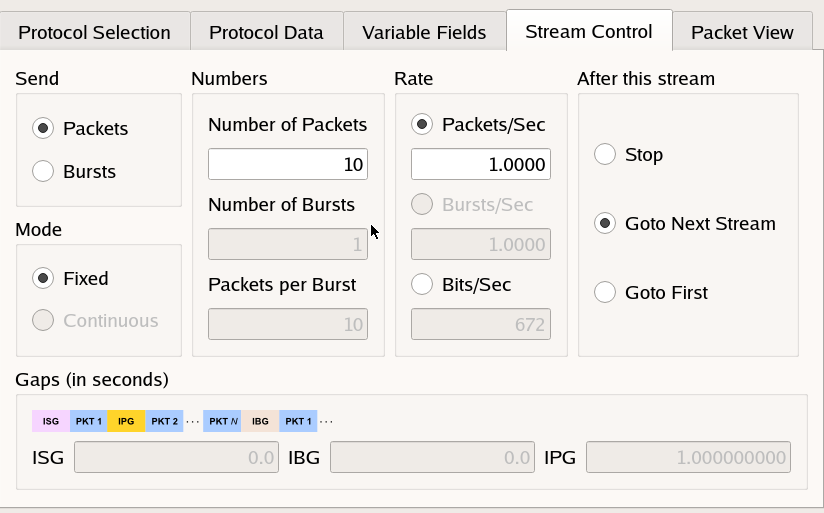
\includegraphics[width=10cm]{data/q2.1-stream-settings.png}
\caption{The stream settings in Ostinato for Question 2.1.}
\label{fig:stream-settings-q2.1}
\end{figure}

As can be seen in Figure \ref{fig:stream-settings-q2.1} the
number of packets, specifically requests, was precisely set
to 10.

\end{ans}

\newpage

\Que{2.2}{Write down the numbers (leftmost column) of the packets that have been generated by:
\begin{itemize}
\item the packet generator
\item the DUT
\end{itemize}
}

\begin{ans}
The required values can be read from Table
\ref{longtable:wireshark-cap-q2.1}.

486, 488, 490, 492, 494, 496, 500, 502, 504 and 506 are the
numbers associated with the request packets generated by
Ostinato.

487, 489, 491, 493, 495, 497, 501, 503, 505 and 507 are the
numbers associated with the reply packets sent by the DUT.
\end{ans}

\Que{2.3}{Use your answer to 2.2 to find the average
inter-packet delay for the packets generated by the packet
generator.}
\begin{ans}

$$
\begin{aligned}
          & \frac{
\begin{aligned}
    & (4618.638764 - 4617.638757)
+(4619.638761 - 4618.638764)
+(4620.638772 - 4619.638761)      \\
+\  & (4621.638731 - 4620.638772)
+(4622.638714 - 4621.638731)
+(4623.638729 - 4622.638714)      \\
+\  & (4624.638727 - 4623.638729)
+(4625.638735 - 4624.638727)
+(4626.638725 - 4625.638735)
\end{aligned}
}{10 - 1}                                      \\
=\        & 0.9999964444444535\ \text{seconds} \\
\approx\  & 1\ \text{seconds}
\end{aligned}
$$

The above computed value is the average inter-packet delay
(in seconds). The approximate value of the above result is 1 second.
This is precisely what was set in the stream's settings (see
Figure \ref{fig:stream-settings-q2.1}).

\begin{gruvboxlisting}[language=Python, caption={Python
expression for calculating the inter-packet delay for
Question 2.3.}]
((4618.638764 - 4617.638757)
+(4619.638761 - 4618.638764)
+(4620.638772 - 4619.638761)
+(4621.638731 - 4620.638772)
+(4622.638714 - 4621.638731)
+(4623.638729 - 4622.638714)
+(4624.638727 - 4623.638729)
+(4625.638735 - 4624.638727)
+(4626.638725 - 4625.638735))/9
\end{gruvboxlisting}

\end{ans}

\newpage

\Que{3}{Repeat the exercises of question 2 with the new packet
rate (2 pkt/s).}

\begin{ans}
\begin{figure}[H]
\centering
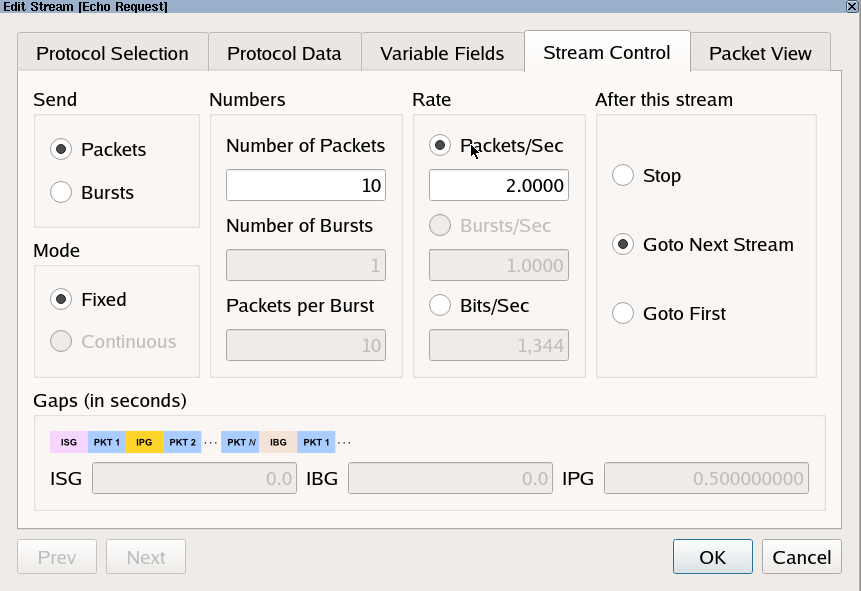
\includegraphics[width=10cm]{data/q3-stream-settings.png}
\caption{The stream settings in Ostinato for Question 3}
\label{fig:stream-settings-q3}
\end{figure}

\begin{center}
\begin{longtable}{|l|l|l|l|l|l|p{\INFOCOLSIZE}|}
\caption{Wireshark ICMP capture for Question 3.}
\label{longtable:wireshark-cap-q3}                                                                             \\
\hline
\multicolumn{1}{|c|}{\textbf{No.}}        &
\multicolumn{1}{c|}{\textbf{Time}}        &
\multicolumn{1}{c|}{\textbf{Source}}      &
\multicolumn{1}{c|}{\textbf{Destination}} &
\multicolumn{1}{c|}{\textbf{Protocol}}    &
\multicolumn{1}{c|}{\textbf{Length}}      &
\multicolumn{1}{c|}{\textbf{Info}}                                                                             \\
\hline
\endfirsthead

\multicolumn{7}{c}{\tablename\ \thetable{} -- continued from previous page}                                    \\
\hline
\multicolumn{1}{|c|}{\textbf{No.}}        &
\multicolumn{1}{c|}{\textbf{Time}}        &
\multicolumn{1}{c|}{\textbf{Source}}      &
\multicolumn{1}{c|}{\textbf{Destination}} &
\multicolumn{1}{c|}{\textbf{Protocol}}    &
\multicolumn{1}{c|}{\textbf{Length}}      &
\multicolumn{1}{c|}{\textbf{Info}}                                                                             \\
\hline
\endhead

\hline
\multicolumn{7}{|c|}{{continued on next page}}                                                                 \\
\hline
\endfoot

\hline
\hline
\endlastfoot

16 & 140.926179 & 192.168.0.10 & 192.168.0.1 & ICMP & 60 & Echo (ping)
request id=0x04d2, seq=0/0, ttl=127 (reply in 17)                                                              \\
17 & 140.926306 & 192.168.0.1 & 192.168.0.10 & ICMP & 60 & Echo (ping)
reply id=0x04d2, seq=0/0, ttl=64 (request in 16)                                                               \\
18 & 141.426171 & 192.168.0.10 & 192.168.0.1 & ICMP & 60 & Echo (ping)
request id=0x04d2, seq=0/0, ttl=127 (reply in 19)                                                              \\
19 & 141.426320 & 192.168.0.1 & 192.168.0.10 & ICMP & 60 & Echo (ping)
reply id=0x04d2, seq=0/0, ttl=64 (request in 18)                                                               \\
20 & 141.926165 & 192.168.0.10 & 192.168.0.1 & ICMP & 60 & Echo (ping)
request id=0x04d2, seq=0/0, ttl=127 (reply in 21)                                                              \\
21 & 141.926287 & 192.168.0.1 & 192.168.0.10 & ICMP & 60 & Echo (ping)
reply id=0x04d2, seq=0/0, ttl=64 (request in 20)                                                               \\
22 & 142.426145 & 192.168.0.10 & 192.168.0.1 & ICMP & 60 & Echo (ping)
request id=0x04d2, seq=0/0, ttl=127 (reply in 23)                                                              \\
23 & 142.426254 & 192.168.0.1 & 192.168.0.10 & ICMP & 60 & Echo (ping)
reply id=0x04d2, seq=0/0, ttl=64 (request in 22)                                                               \\
24 & 142.926106 & 192.168.0.10 & 192.168.0.1 & ICMP & 60 & Echo (ping)
request id=0x04d2, seq=0/0, ttl=127 (reply in 25)                                                              \\
25 & 142.926275 & 192.168.0.1 & 192.168.0.10 & ICMP & 60 & Echo (ping)
reply id=0x04d2, seq=0/0, ttl=64 (request in 24)                                                               \\
26 & 143.426150 & 192.168.0.10 & 192.168.0.1 & ICMP & 60 & Echo (ping)
request id=0x04d2, seq=0/0, ttl=127 (reply in 27)                                                              \\
27 & 143.426249 & 192.168.0.1 & 192.168.0.10 & ICMP & 60 & Echo (ping)
reply id=0x04d2, seq=0/0, ttl=64 (request in 26)                                                               \\
28 & 143.926104 & 192.168.0.10 & 192.168.0.1 & ICMP & 60 & Echo (ping)
request id=0x04d2, seq=0/0, ttl=127 (reply in 29)                                                              \\
29 & 143.926259 & 192.168.0.1 & 192.168.0.10 & ICMP & 60 & Echo (ping)
reply id=0x04d2, seq=0/0, ttl=64 (request in 28)                                                               \\
30 & 144.426138 & 192.168.0.10 & 192.168.0.1 & ICMP & 60 & Echo (ping)
request id=0x04d2, seq=0/0, ttl=127 (reply in 31)                                                              \\
31 & 144.426250 & 192.168.0.1 & 192.168.0.10 & ICMP & 60 & Echo (ping)
reply id=0x04d2, seq=0/0, ttl=64 (request in 30)                                                               \\
32 & 144.926075 & 192.168.0.10 & 192.168.0.1 & ICMP & 60 & Echo (ping)
request id=0x04d2, seq=0/0, ttl=127 (reply in 33)                                                              \\
33 & 144.926259 & 192.168.0.1 & 192.168.0.10 & ICMP & 60 & Echo (ping)
reply id=0x04d2, seq=0/0, ttl=64 (request in 32)                                                               \\
34 & 145.426128 & 192.168.0.10 & 192.168.0.1 & ICMP & 60 & Echo (ping)
request id=0x04d2, seq=0/0, ttl=127 (reply in 35)                                                              \\
35 & 145.426236 & 192.168.0.1 & 192.168.0.10 & ICMP & 60 & Echo (ping)
reply id=0x04d2, seq=0/0, ttl=64 (request in 34)                                                               \\
\end{longtable}
\end{center}

Again the number of packets in total is 20. 10 requests and
10 replies as specified in the stream's settings, see
Figure \ref{fig:stream-settings-q3}.

And from Table \ref{longtable:wireshark-cap-q3} we can get
the respective No. of the request and reply packets

The request packets are precisely numbers: 16, 18, 20, 22,
24, 26, 28, 30, 32, 34.

And the reply packets are precisely numbers: 17, 19, 21,
23, 25, 27, 29, 31, 33, 35.

Finally, the below computed value is the average
inter-packet delay (in seconds).

$$
\begin{aligned}
          & \frac{
\begin{aligned}
    & (141.426171 - 140.926179)
+(141.926165 - 141.426171)
+(142.426145 - 141.926165)      \\
+\  & (142.926106 - 142.426145)
+(143.426150 - 142.926106)
+(143.926104 - 143.426150)      \\
+\  & (144.426138 - 143.926104)
+(144.926075 - 144.426138)
+(145.426128 - 144.926075)
\end{aligned}
}{10 - 1}                                     \\
=\        & 0.499994333333335\ \text{seconds} \\
\approx\  & 0.5\ \text{seconds}
\end{aligned}
$$

The approximate value of the above result is 0.5 seconds. This
is precisely what should be expected since if two request are
being sent per second (see Figure \ref{fig:stream-settings-q3})
that would equate to a request every half a second.

\begin{gruvboxlisting}[language=Python,caption={Python
expression for calculating the inter-packet delay for
Question 3.}]
((141.426171 - 140.926179)
+(141.926165 - 141.426171)
+(142.426145 - 141.926165)
+(142.926106 - 142.426145)
+(143.426150 - 142.926106)
+(143.926104 - 143.426150)
+(144.426138 - 143.926104)
+(144.926075 - 144.426138)
+(145.426128 - 144.926075))/9
\end{gruvboxlisting}
\end{ans}

\Que{4.1}{Expand the frame section and inspect it to find out
the number of bytes captured by Wireshark from the link (``bytes
on wire'').}

\begin{ans}
\begin{figure}[H]
\centering
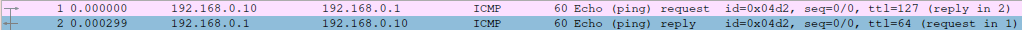
\includegraphics[width=16cm]{data/q4.1-packets-under-inspection.png}
\caption{The packets under inspection for Question 4.1.}
\end{figure}

The info related to the request from the generator to the
DUT is provided below. Specifically, the information
related to the Ethernet II frame.

\begin{figure}[H]
\centering
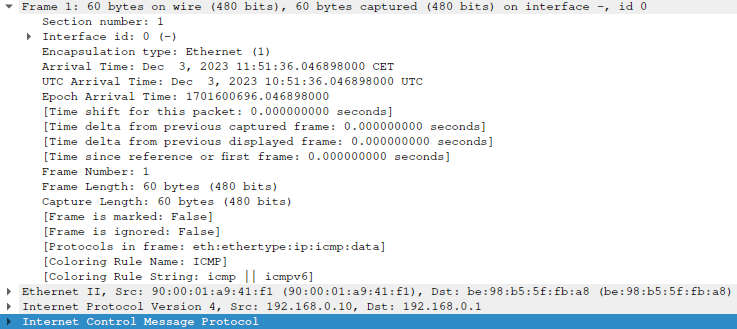
\includegraphics[width=16cm]{data/q4.1-request-info.png}
\caption{The frame information of the request packet under
insception for Question 4.1.}
\end{figure}

The number of bytes captured by Wireshark is exactly 60 bytes.
\end{ans}

\Que{4.2}{Search for the minimum length of an Ethernet packet,
and state it.}

\begin{ans}
\begin{figure}[H]
\centering
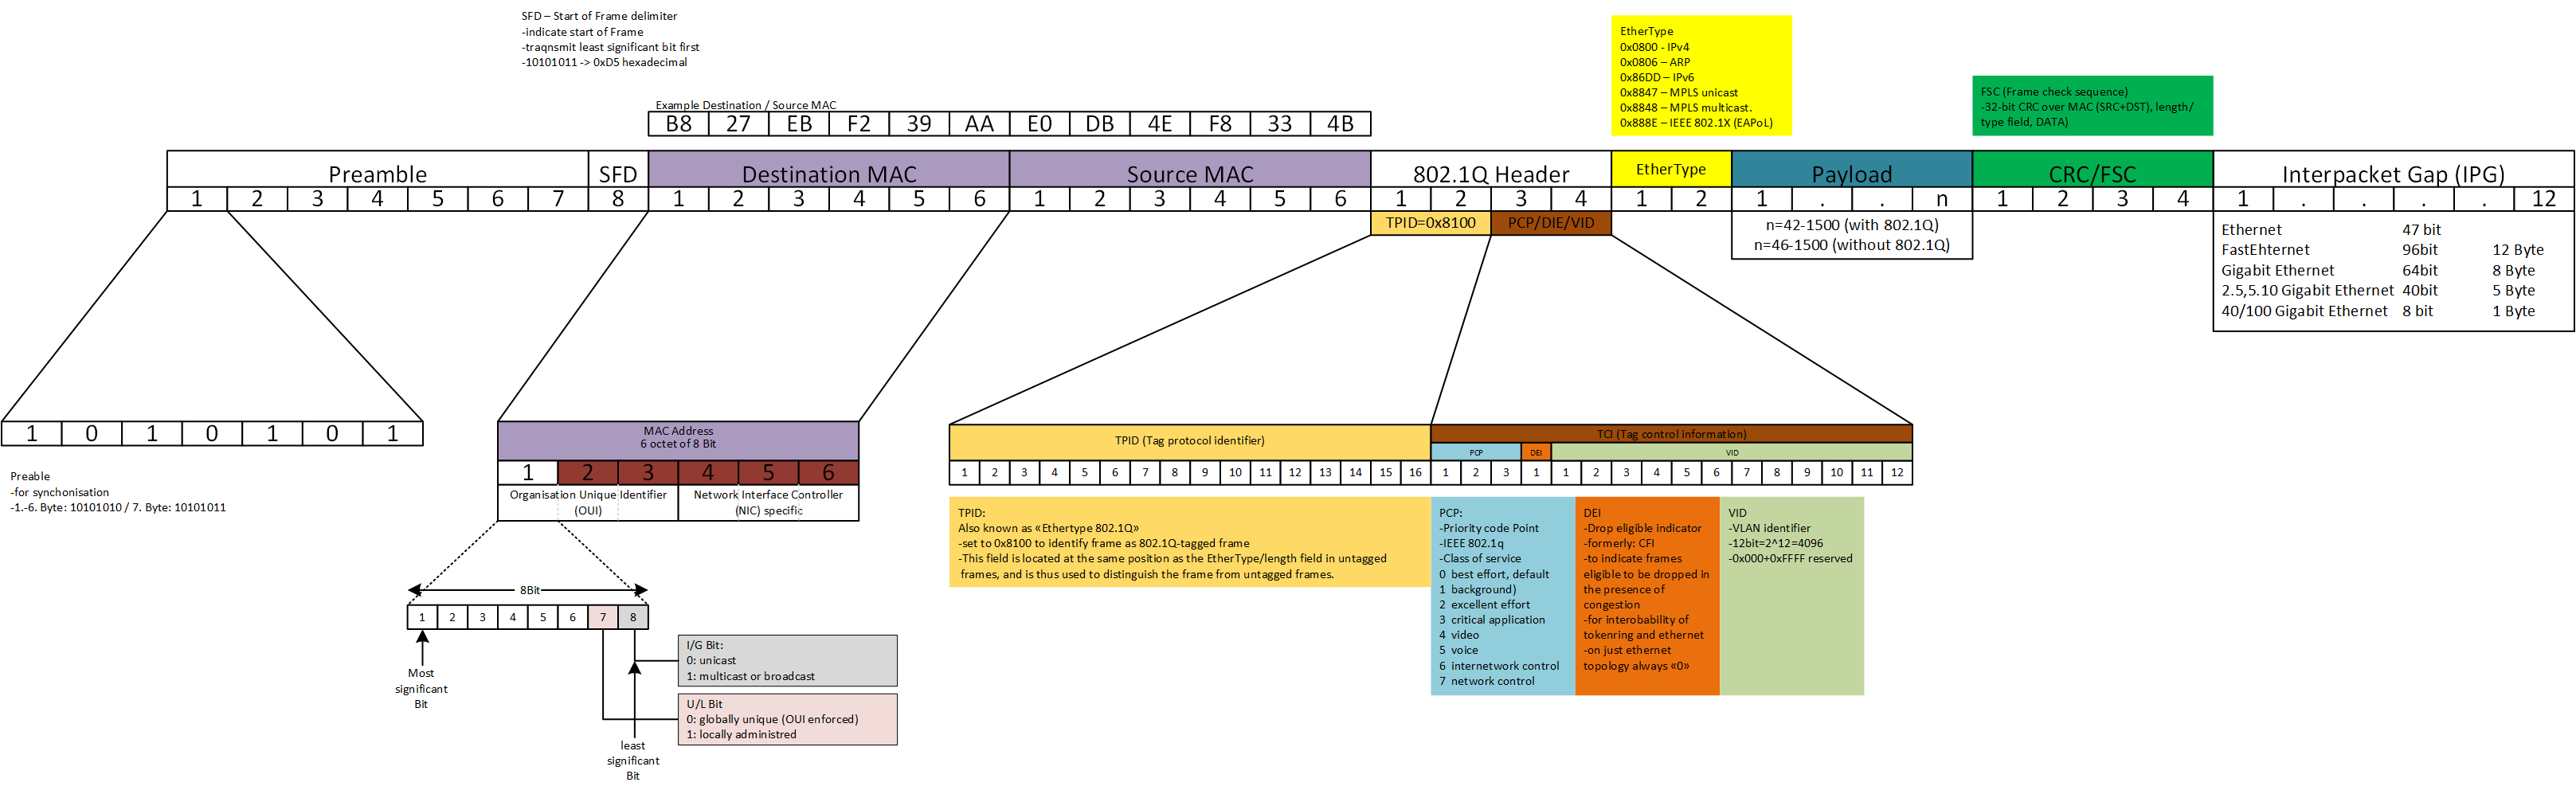
\includegraphics[width=16cm]{data/q4.2-ethernet-diagram.png}
\caption{A diagram of the components of an Ethernet II frame.}
\label{fig:eth2-frame}
\end{figure}

\Refer{https://upload.wikimedia.org/wikipedia/commons/7/72/Ethernet_Frame.png}

\begin{note}
There is a mistake in the graphic. ``CRC/FSC'' should be
``CRC/FCS'' and ``FSC (Frame check sequence)'' should be ``FCS
(Frame check sequence)''.
\end{note}

The minimum and maximum lengths can be derived from Figure
\ref{fig:eth2-frame}. Importantly, the preamble, SFD and
inter-pack gap are almost never exposed beyond layer 1.
Therefore, we shall not factor these into our calculation.

Hence, the Ethernet II frame at layer 2 consists of the
following segments:

\begin{itemize}
\item Destination MAC (6 octets);
\item Source MAC (6 octets);
\item 802.1Q Header (optional \& 4 octets);
\item EtherType (2 octets);
\item Payload (42 --- 1500 octets with 802.1Q \& 46 --- 1500
      octets without 802.1Q); and
\item CRC/FCS (4 octets).
\end{itemize}

Following this, the minimum length can be calculated as follows:

$$
{\text{Frame}}_{\text{min}} = 6 + 6 + 2 + 46 + 4 = 64\ \text{octets}
$$

\begin{note}
In the case when there is no 802.1Q header, the total header and
payload lengths add up to 46. This is because the header length
is 0 and the payload has a minimum length of 46. In the other
case \ie{} when there is a 802.1Q header, the total header and
payload lengths also add up to 46. This is because the header
length is 4 and the payload length has a new minimum of 42,
since 4 have already been used by 802.1Q header. Hence, in both
cases the sum of their lengths is identical.
\end{note}

Similarly, the maximum length is given by the following
calculation:

$$
{\text{Frame}}_{\text{max}} = 6 + 6 + 2 + 1500 + 4 = 1518\ \text{octets}
$$
\end{ans}

\Que{4.3}{How does the number of bytes captured (which you found
in (4.1)) compare with the minimum length of an Ethernet packet
(which you looked up in (4.2))? Can you explain the difference?}

\begin{ans}
\begin{figure}[H]
\centering
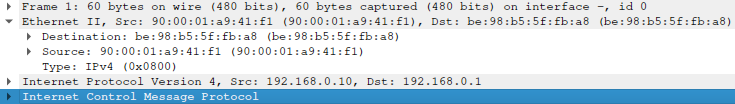
\includegraphics[width=14cm]{data/q4.3-ethernet-header.png}
\caption{The Ethernet II header of the request packet under
inspection for Question 4.1.}
\label{fig:eth2-header-for-q4.3}
\end{figure}

The number of ``bytes on wire'' according to Wireshark (see
Figure \ref{fig:eth2-header-for-q4.3}) is precisely 60 bytes.
However, the minimum number of bytes is at least 64.

To account for the 4 byte, notice that the Ethernet II header
does not contain an 802.1Q header. Hence, the payload is allowed
a minimum of 46 bytes. Additionally, all these 46 bytes are used
up by the ICMP request (including all IP overhead).

Hence, the Ethernet header and ICMP request sum up to 60 bytes.
This leaves only one option as to what the remaining 4 bytes can
be. They constitute the Cyclic Redundancy Check (CRC) or Frame
Check Sequence (FCS). In fact, according to Figure
\ref{fig:eth2-frame}, the CRC field is exactly 4 bytes.

Furthermore, this conclusion is supported by the
below referenced Wireshark forum discussion. One of the
users exclaims that ``bytes on wire'' is often more like
``bytes on wire without CRC''.

This is the case because a CRC fails, the network driver which
performs the check will often automatically drop the invalid
packet. This mean that invalid packets will never actually reach
user space. Hence, providing the CRC to user space applications
is often a redundant since the CRC would have already been
checked to be vaild.

\Refer{https://osqa-ask.wireshark.org/questions/1344/does-frame-length-include-also-crc-bytes}
\end{ans}

\Que{4.4}{Expand the Ethernet II section and write down the
source MAC address and the destination MAC address.}

\begin{ans}
Source MAC = \texttt{90:00:01:a9:41:f1}

Destination MAC = \texttt{be:98:b5:5f:fb:a8}

The above where taken from Figure
\ref{fig:eth2-header-for-q4.3}.
\end{ans}

\Que{4.5}{Look up the source MAC address in the device group
configured on the packet generator at the port group.}

\begin{ans}
\begin{figure}[H]
\centering
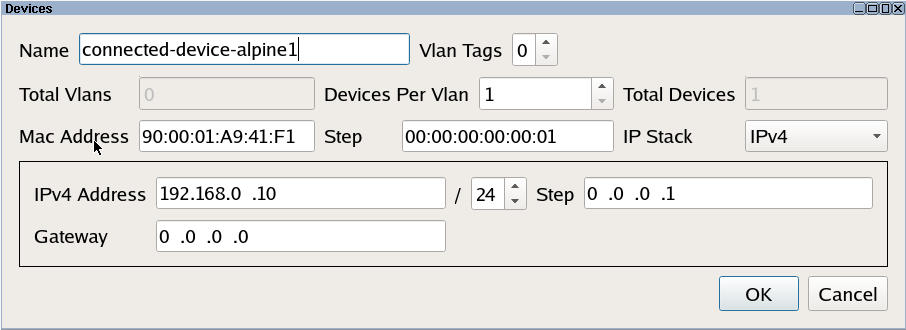
\includegraphics[width=14cm]{data/q4.5-device-group-config.png}
\caption{The device group configuration in Ostinator for
Question 4.5.}
\label{fig:devic-config-q4.5}
\end{figure}
\begin{note}
Since the device group contains as single device the
base MAC address \ie{} \texttt{90:00:01:a9:41:f1} is used for that
device.
\end{note}

As can be seen in Figure \ref{fig:devic-config-q4.5}, the
device is given the MAC address \texttt{90:00:01:a9:41:f1}.
\end{ans}

\Que{4.6}{Compare what was found in 4.4 with what was found in
4.5.}
\begin{ans}
\begin{note}
Assuming that in the original question, 5.4 and 5.5 were
meant to be 4.4 and 4.5 respectively.
\end{note}

As expected, the MAC address of the virtual device is
identical to the source MAC Address in the packet. This is
because the packet is a request packet \ie{} it was created
by Ostinato.

It is also critical to notice that any form of local layer 3
communication is very much dependent on ARP. This is because ARP
facilitates layer 3 communication over layer 2. It does this by
providing the capability to resolve \ie{} find the MAC address
of an IP address holder.

\begin{note}
In this context the ``local'' layer 3 network of a device is all
the other devices which have the same network address and are
reachable via layer 2.
\end{note}
\end{ans}

\Que{4.7}{Inspect the Ethernet II section and find the field in
that section which the receiver (the DUT) uses to identify the
layer 3 entity which is to receive the Ethernet frame's
payload.}
\begin{ans}
In Question 4.2 the EtherType field is referenced. The
EtherType field specifies what type of payload the
Ethernet frame contains. The EtherType in the frame of
interest is set to \texttt{0x0800}, see Figure
\ref{fig:eth2-header-for-q4.3}. \texttt{0x0800}
identifies the payload inside the frame as an IPv4
packet. This gives the DUT the required information to
properly decode the contents of the payload.
\end{ans}

\newpage

\Que{4.8}{Inspect the section below the Ethernet II section and:
\begin{itemize}
\item write down the source address and the destination address
      that you see in this underlying section;
\item compare the source address and the destination address with
      what you have set up in the stream named ``ICMP Echo
      Request Stream''.
\item Look up the field named ``Total length'' in this section
      and account for the difference between this number and the
      number you have found in 4.1.
\end{itemize}}

\begin{ans}
\begin{figure}[H]
\centering
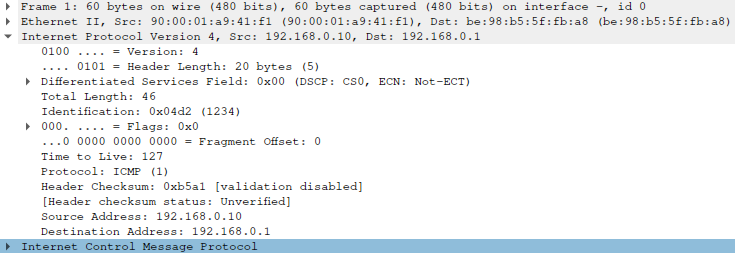
\includegraphics[width=14cm]{data/q4.8-ip-header.png}
\caption{The IPv4 header of the request packet under
inspection for Question 4.1.}
\label{fig:ip-header-for-q4.8}
\end{figure}

Source IP Address = \texttt{192.168.0.10}

Destination IP Address = \texttt{192.168.0.1}

See Figure \ref{fig:ip-header-for-q4.8} to verify the above
addresses.

\begin{figure}[H]
\centering
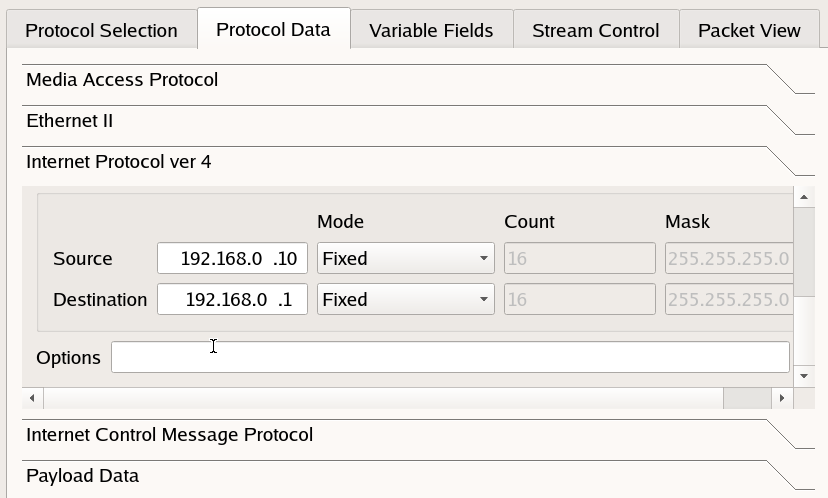
\includegraphics[width=14cm]{data/q4.8-stream-config.png}
\caption{The stream's IPv4 configuration in Ostinato for Question 4.8.}
\label{fig:stream-config-for-q4.8}
\end{figure}

Additionally, the Total Length is 46 bytes, again see
Figure \ref{fig:ip-header-for-q4.8}. This is precisely what
was described in Question 4.3. Again, the Ethernet header
length is 14 bytes, and $14 + 46 = 60$ bytes as expected.

Additionally, 20 of the 46 bytes are the IPv4 Header Length
whilst the remaining 26 bytes are the actual ICMP Request.
\end{ans}

\newpage

\Que{5}{For each packet, state source and destination IPv4
address. Compare these latter two addresses with the IPv4
address bound to alpine-1 eth0, and justify the outcome of your
comparison.}

\begin{ans}
\begin{figure}[H]
\centering
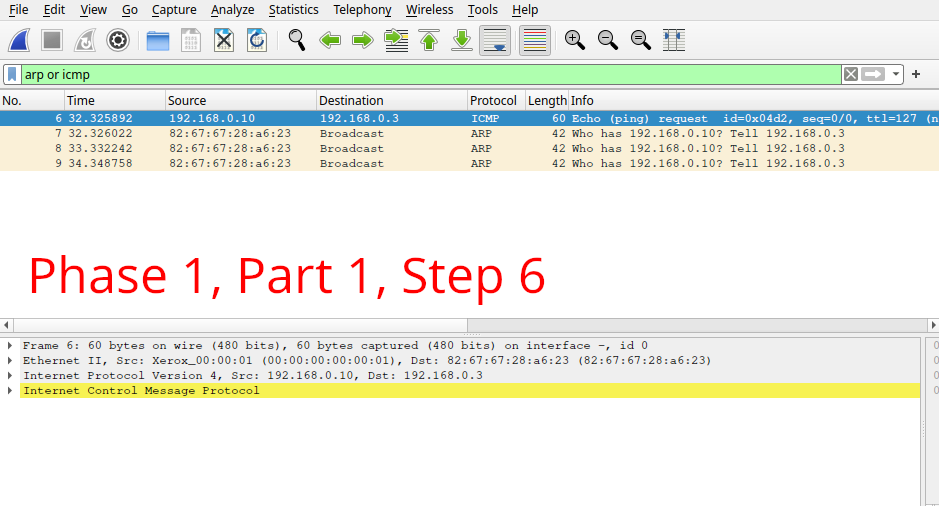
\includegraphics[width=14cm]{data/q5-capture1.png}
\caption{The Wireshark capture for phase 1, part 1, step 6.}
\label{fig:wireshark-capture1-q5}
\end{figure}

\begin{figure}[H]
\centering
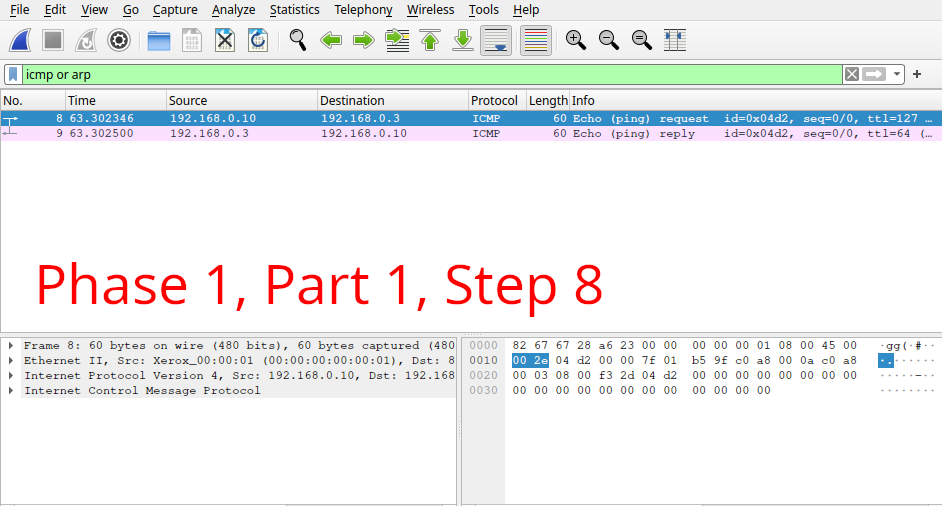
\includegraphics[width=14cm]{data/q5-capture2.png}
\caption{The Wireshark capture for phase 1, part 1, step 8.}
\label{fig:wireshark-capture2-q5}
\end{figure}

\begin{figure}[H]
\centering
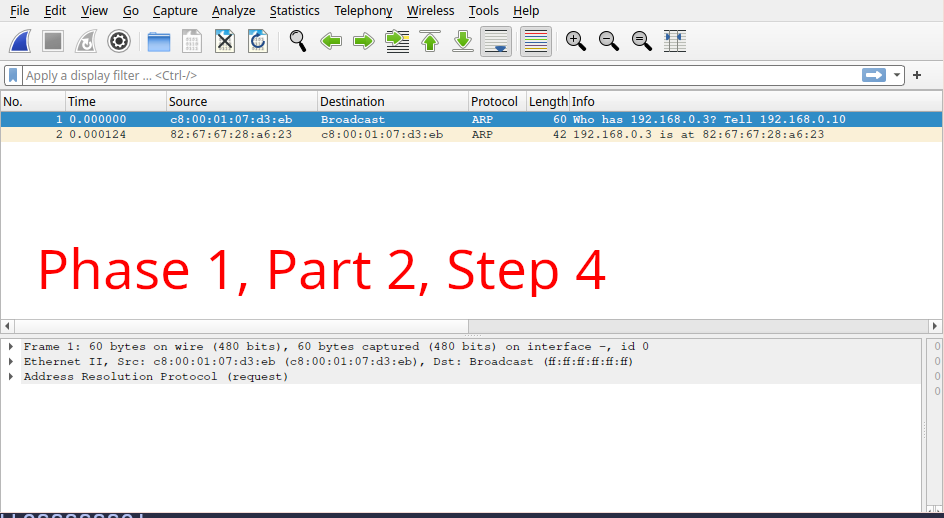
\includegraphics[width=14cm]{data/q5-capture3.png}
\caption{The Wireshark capture for phase 1, part 2, step 4.}
\label{fig:wireshark-capture3-q5}
\end{figure}

\begin{figure}[H]
\centering
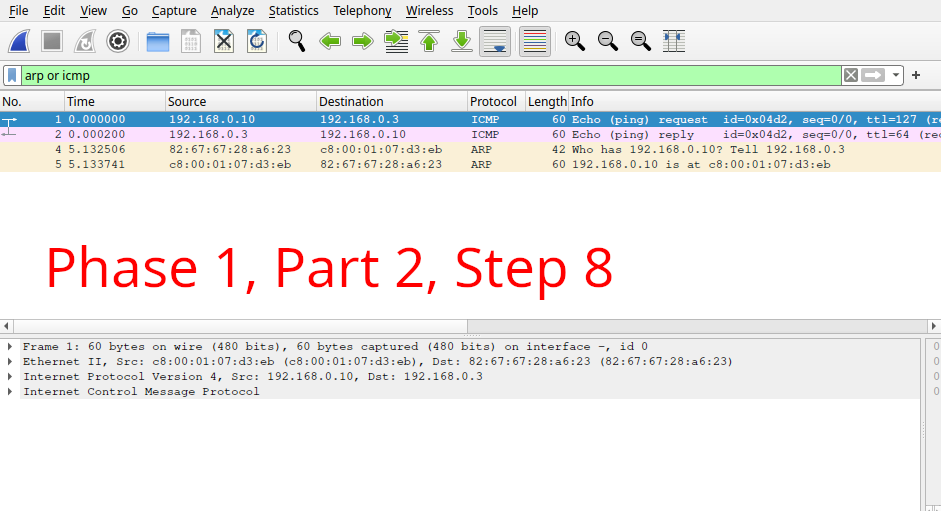
\includegraphics[width=14cm]{data/q5-capture4.png}
\caption{The Wireshark capture for phase 1, part 2, step 8.}
\label{fig:wireshark-capture4-q5}
\end{figure}

The above four pictures are all the Wireshark captures as
specified in the lab sheet.

As can be seen from Figure \ref{fig:wireshark-capture1-q5}, the
IP addresses in use are \texttt{192.168.0.10} and
\texttt{192.168.0.3}. These are the IP addresses of the virtual
Ostinatio devices and alpine-3 respectively.

\begin{note}
All the captures in Figures \ref{fig:wireshark-capture1-q5},
\ref{fig:wireshark-capture2-q5}, \ref{fig:wireshark-capture3-q5}
\& \ref{fig:wireshark-capture4-q5} were made over Hub1
$\leftrightarrow$ alpine-1. This exposes the nature of hubs as
networking devices. Hubs do not keep track of any form of source
to/from destination map. Hubs take a broad stroke approach and
replay any communication they receive into all of their other
connections.
\end{note}
\end{ans}

\Que{6}{Compare the packet(s) you capture on Switch1
$\leftrightarrow$ alpine-2. State at least one difference
between your output and that shown in Fig. 37, and explain it.}

\begin{ans}
For this question all the steps described in Phase 1, Part 2
were repeated. However, this time Port 1 (in Ostinato) was used
and connections Switch1 $\leftrightarrow$ apline-2 and Swtich1
$\leftrightarrow$ apline-4 were monitored.

\begin{figure}[H]
\centering
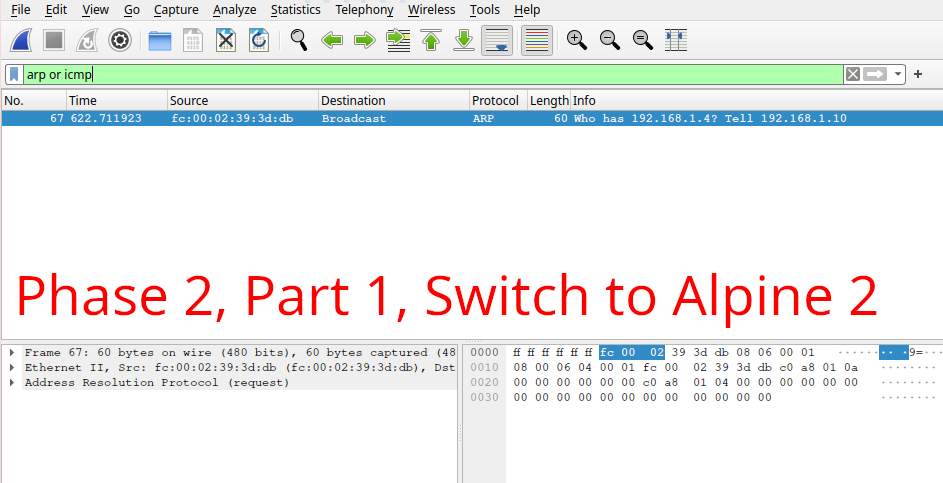
\includegraphics[width=14cm]{data/q6-phase2-switch-to-alpine2-part1.png}
\caption{The Wireshark capture for phase 2, part 1 on connection Switch1 $\leftrightarrow$ alpine-2.}
\label{fig:wireshark-phase2-part1-for-q6}
\end{figure}

\begin{figure}[H]
\centering
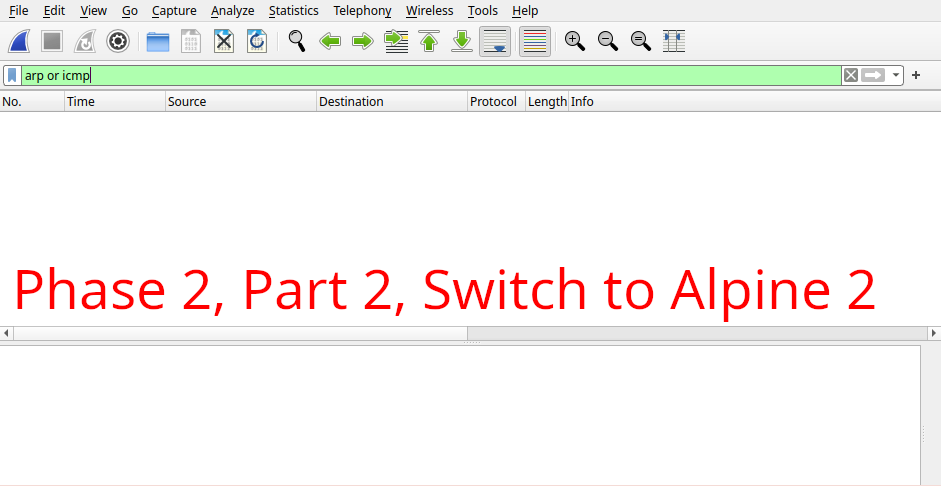
\includegraphics[width=14cm]{data/q6-phase2-switch-to-alpine2-part2.png}
\caption{The Wireshark capture for phase 2, part 2 on connection Switch1 $\leftrightarrow$ alpine-2.}
\label{fig:wireshark-phase2-part2-for-q6}
\end{figure}

Firstly, it is important to note that only a single packet is
captured on the Switch1 $\leftrightarrow$ alpine-2 connection,
see Figure \ref{fig:wireshark-phase2-part1-for-q6} and
\ref{fig:wireshark-phase2-part2-for-q6}.

Additionally, the only difference between the ARP packet in
Figure \ref{fig:wireshark-phase2-part1-for-q6} and the ARP
packet in Fig. 37 (of the lab sheet) is the MAC address.

\begin{note}
The documented difference is not very meaningful. This is
because Ostinato provides the facility to manually specify the
MAC addresses of its virtual devices. Hence, with a little bit
of care to ensure no MAC address collisions, the same result as
Fig. 37 can be achieved.
\end{note}
\end{ans}

\newpage

\Que{7.1}{Present a screenshot that shows the packets you have
captured on Switch1 $\leftrightarrow$ alpine-4.}

\begin{ans}
\begin{figure}[H]
\centering
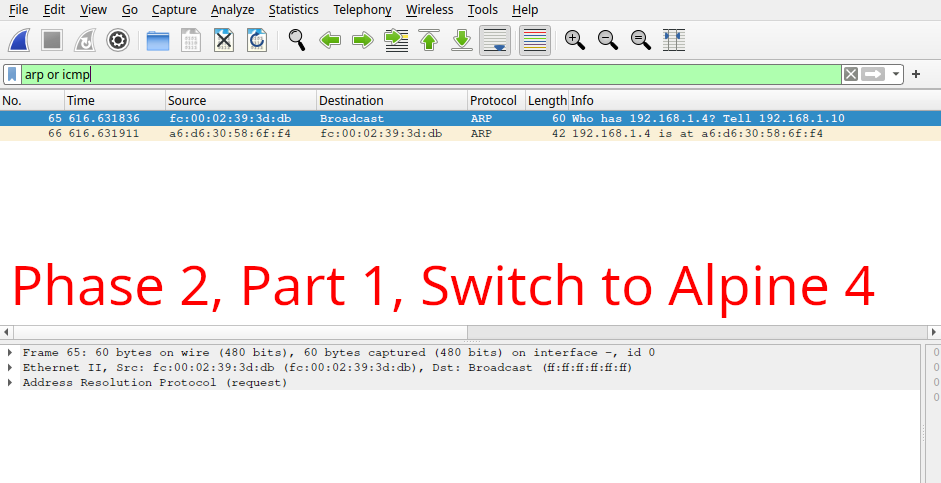
\includegraphics[width=14cm]{data/q6-phase2-switch-to-alpine4-part1.png}
\caption{The Wireshark capture for phase 2, part 1 on connection Switch1 $\leftrightarrow$ alpine-4.}
\label{fig:wireshark-phase2-part1-for-q6-conn2}
\end{figure}

\begin{figure}[H]
\centering
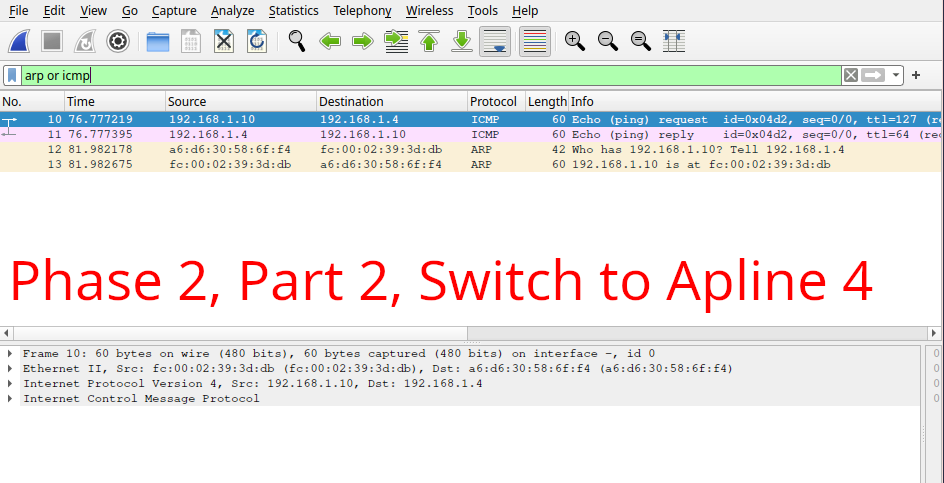
\includegraphics[width=14cm]{data/q6-phase2-switch-to-alpine4-part2.png}
\caption{The Wireshark capture for phase 2, part 2 on connection Switch1 $\leftrightarrow$ alpine-4.}
\label{fig:wireshark-phase2-part2-for-q6-conn2}
\end{figure}
\end{ans}

\Que{7.2}{For each packet, explain how it fits into the sequence
that is generated as a result of running the packet stream you
have configured on Ostinato.}

\begin{ans}
From here on-wards the packets in Figures
\ref{fig:wireshark-phase2-part1-for-q6-conn2} and
\ref{fig:wireshark-phase2-part2-for-q6-conn2} will be refered to
with there number (labelled `No.' in the Figures). Specifically,
these are: 65, 66 and 10, 11, 12, 13.

\begin{itemize}
\item No. 65 and No. 66 constitute the first ARP correspondence
    initiated by applying the stream configuration in Ostinato.
    ARP is used to establish whether the entity associated with
    the specified IP address, is also an L2 entity in the local
    network. Additionally, if the entity is an L2 entity it
    replies back with its MAC address. This procedure happens
    via an initial request for discovery. In the above case this
    request is No. 65. The device initiating ARP will broadcast
    an ARP packet inquiring about the MAC Address of the current
    holder of the specified IP. Each device on the local network
    will receive this ARP packet. Each device will then proceed
    to check whether they hold the requested IP address. If they
    do they will send their MAC address as a uni-cast ARP
    packet, since the MAC address of the initiator is known. In
    the above case this is reply No. 66.
\item No. 10 and No. 11 are the ICMP Echo request/reply pair The
    request (No. 10), is sent when the configured Ostinato
    stream is run. The reply (No. 11) is sent by the receiver of
    the request to inform the initiating device (in this case an
    Ostinato virtual device) that it is available and ready to
    serve.
    \begin{note}
    Pings (ICMP Echo Requests) are meant to check whether a
    device with a specified IP address exists and whether it can
    service requests. This can be observed in Figure
    \ref{fig:wireshark-phase2-part2-for-q6-conn2}.
    \end{note}
\item No. 12 and No. 13 constitute the ARP correspondence which
    was autonomously initiated by apline-4 as described in the
    lab sheet.
\end{itemize}
\end{ans}

\newpage

\Que{7.3}{Select the ICMP packet generated by Ostinato. Use a
tabular structure, exemplified by Fig. 39, to name
\textbf{all} the fields, for all the layers, in the ICMP
packet. For each field name, write a prefix to indicate
which layer the field pertains to, e.g., L1 for layer 1,
L2 for layer 2, etc.}

\begin{ans}

\begin{figure}[H]
\begin{subfigure}[c]{0.73\textwidth}
\centering
\begin{adjustbox}{width=\linewidth}
\begin{bytefield}[bitwidth=1.5em,bitheight=2.6em]{32}
\bitheader{0-31} \\
\wordbox[tlr]{1}[bgcolor=pastelblue]{L2: Destination MAC\textsubscript{48}} \\
\bitbox[blr]{16}[bgcolor=pastelblue]{} & \bitbox[tlr]{16}[bgcolor=pastelblue]{} \\
\wordbox[lr]{1}[bgcolor=pastelblue]{L2: Source MAC\textsubscript{48}} \\
\bitbox{16}[bgcolor=pastelblue]{L2: EtherType\textsubscript{16}} &
\bitbox{16}[bgcolor=pastelgrey]{} \\
\bitbox{4}[bgcolor=pastelgreen]{L3: Version\textsubscript{4}} &
\bitbox{4}[bgcolor=pastelgreen]{\footnotesize L3: Header Length\textsubscript{4}} &
\bitbox{6}[bgcolor=pastelgreen]{L3: DSCP\textsubscript{6}} &
\bitbox{2}[bgcolor=pastelgreen]{\footnotesize L3: ECN\textsubscript{2}} &
\bitbox{16}[bgcolor=pastelgreen]{L3: Total Length\textsubscript{16}} \\
\bitbox{16}[bgcolor=pastelgreen]{L3: Identification\textsubscript{16}} &
\bitbox{3}[bgcolor=pastelgreen]{L3: Flags\textsubscript{3}} &
\bitbox{13}[bgcolor=pastelgreen]{L3: Fragment Offset\textsubscript{13}} \\
\bitbox{8}[bgcolor=pastelgreen]{L3: TTL\textsubscript{8}} &
\bitbox{8}[bgcolor=pastelgreen]{L3: Protocol\textsubscript{8}} &
\bitbox{16}[bgcolor=pastelgreen]{L3: Header Checksum\textsubscript{16}} \\
\wordbox{1}[bgcolor=pastelgreen]{L3: Source Address\textsubscript{32}}\\
\wordbox{1}[bgcolor=pastelgreen]{L3: Destination Address\textsubscript{32}}\\
\bitbox{8}[bgcolor=pastelpink]{L3: Type\textsubscript{8}} &
\bitbox{8}[bgcolor=pastelpink]{L3: Code\textsubscript{8}} &
\bitbox{16}[bgcolor=pastelpink]{L3: Checksum\textsubscript{16}}\\
\bitbox{16}[bgcolor=pastelpink]{L3: Identifier\textsubscript{16}} &
\bitbox{16}[bgcolor=pastelpink]{L3: Sequence Number\textsubscript{16}} \\
\wordbox{1}[bgcolor=pastelpink]{L3: Data\textsubscript{144}} \\
\end{bytefield}
\end{adjustbox}
\end{subfigure}
\hfill
\begin{subfigure}[c]{13em}
\centering
\begin{tabular}{cl}
\legendbox{pastelblue}{} & Ethernet II     \\
\legendbox{pastelgreen}{} & IPv4            \\
\legendbox{pastelpink}{}  & ICMP            \\
\legendbox{pastelgrey}{}  & Diagram Padding \\
\\
\multicolumn{2}{p{13em}}{\small \textbf{MAC} = Media Access Control}\\
\multicolumn{2}{p{13em}}{\small \textbf{DSCP} = Differentiated Services Code Point}\\
\multicolumn{2}{p{13em}}{\small \textbf{ECN} = Explicit Congestion Notification}
\end{tabular}
\end{subfigure}
\caption{A diagram of the structure of an ICMP packet as provided by Wireshark.}
\label{fig:icmp-diagram}
\end{figure}

\begin{note}
The bits marked as ``Diagram Padding'' in Figure
\ref{fig:icmp-diagram} are \emph{only} present to allow for a
properly partitioned diagram, they are \emph{not} present ``on
the wire'', \ie{} all the fields are packed. Additionally, each
field is marked with its respective bit size (as a subscript),
network layer (as ``L$N$:'') and packet type (as a colour).
\end{note}
\end{ans}

\Que{8}{Explain why the packets captured on Switch1
$\leftrightarrow$ alpine-2 do not change between the point in
time just before running the packet stream on Ostinato, and
the point in time just after
running it.}
\begin{ans}
No packets are captured on connection Switch1 $\leftrightarrow$
alpine-2 in phase 2, part 2 (see Figure
\ref{fig:wireshark-phase2-part2-for-q6}). This is because the
switch as a network device keeps a mapping from ports to MAC
addresses and vice-versa. This means it is capable of
selectively replaying packets to their intended recipients
directly. In fact, the rest of the communication is only held on
connection Switch1 $\leftrightarrow$ alpine-4 (see Figure
\ref{fig:wireshark-phase2-part2-for-q6-conn2}).
\end{ans}

\Que{9}{
This concerns the dynamics of transmission using TCP. For each
of the four cases (lossless, and packet loss at the rate of 1\%,
3\% and 5\% respectively):
\begin{enumerate}
\item Plot a 1-s MA of the throughput, and
\item calculate the average throughput
\end{enumerate}}
\begin{ans}

\begin{figure}[H]
\centering
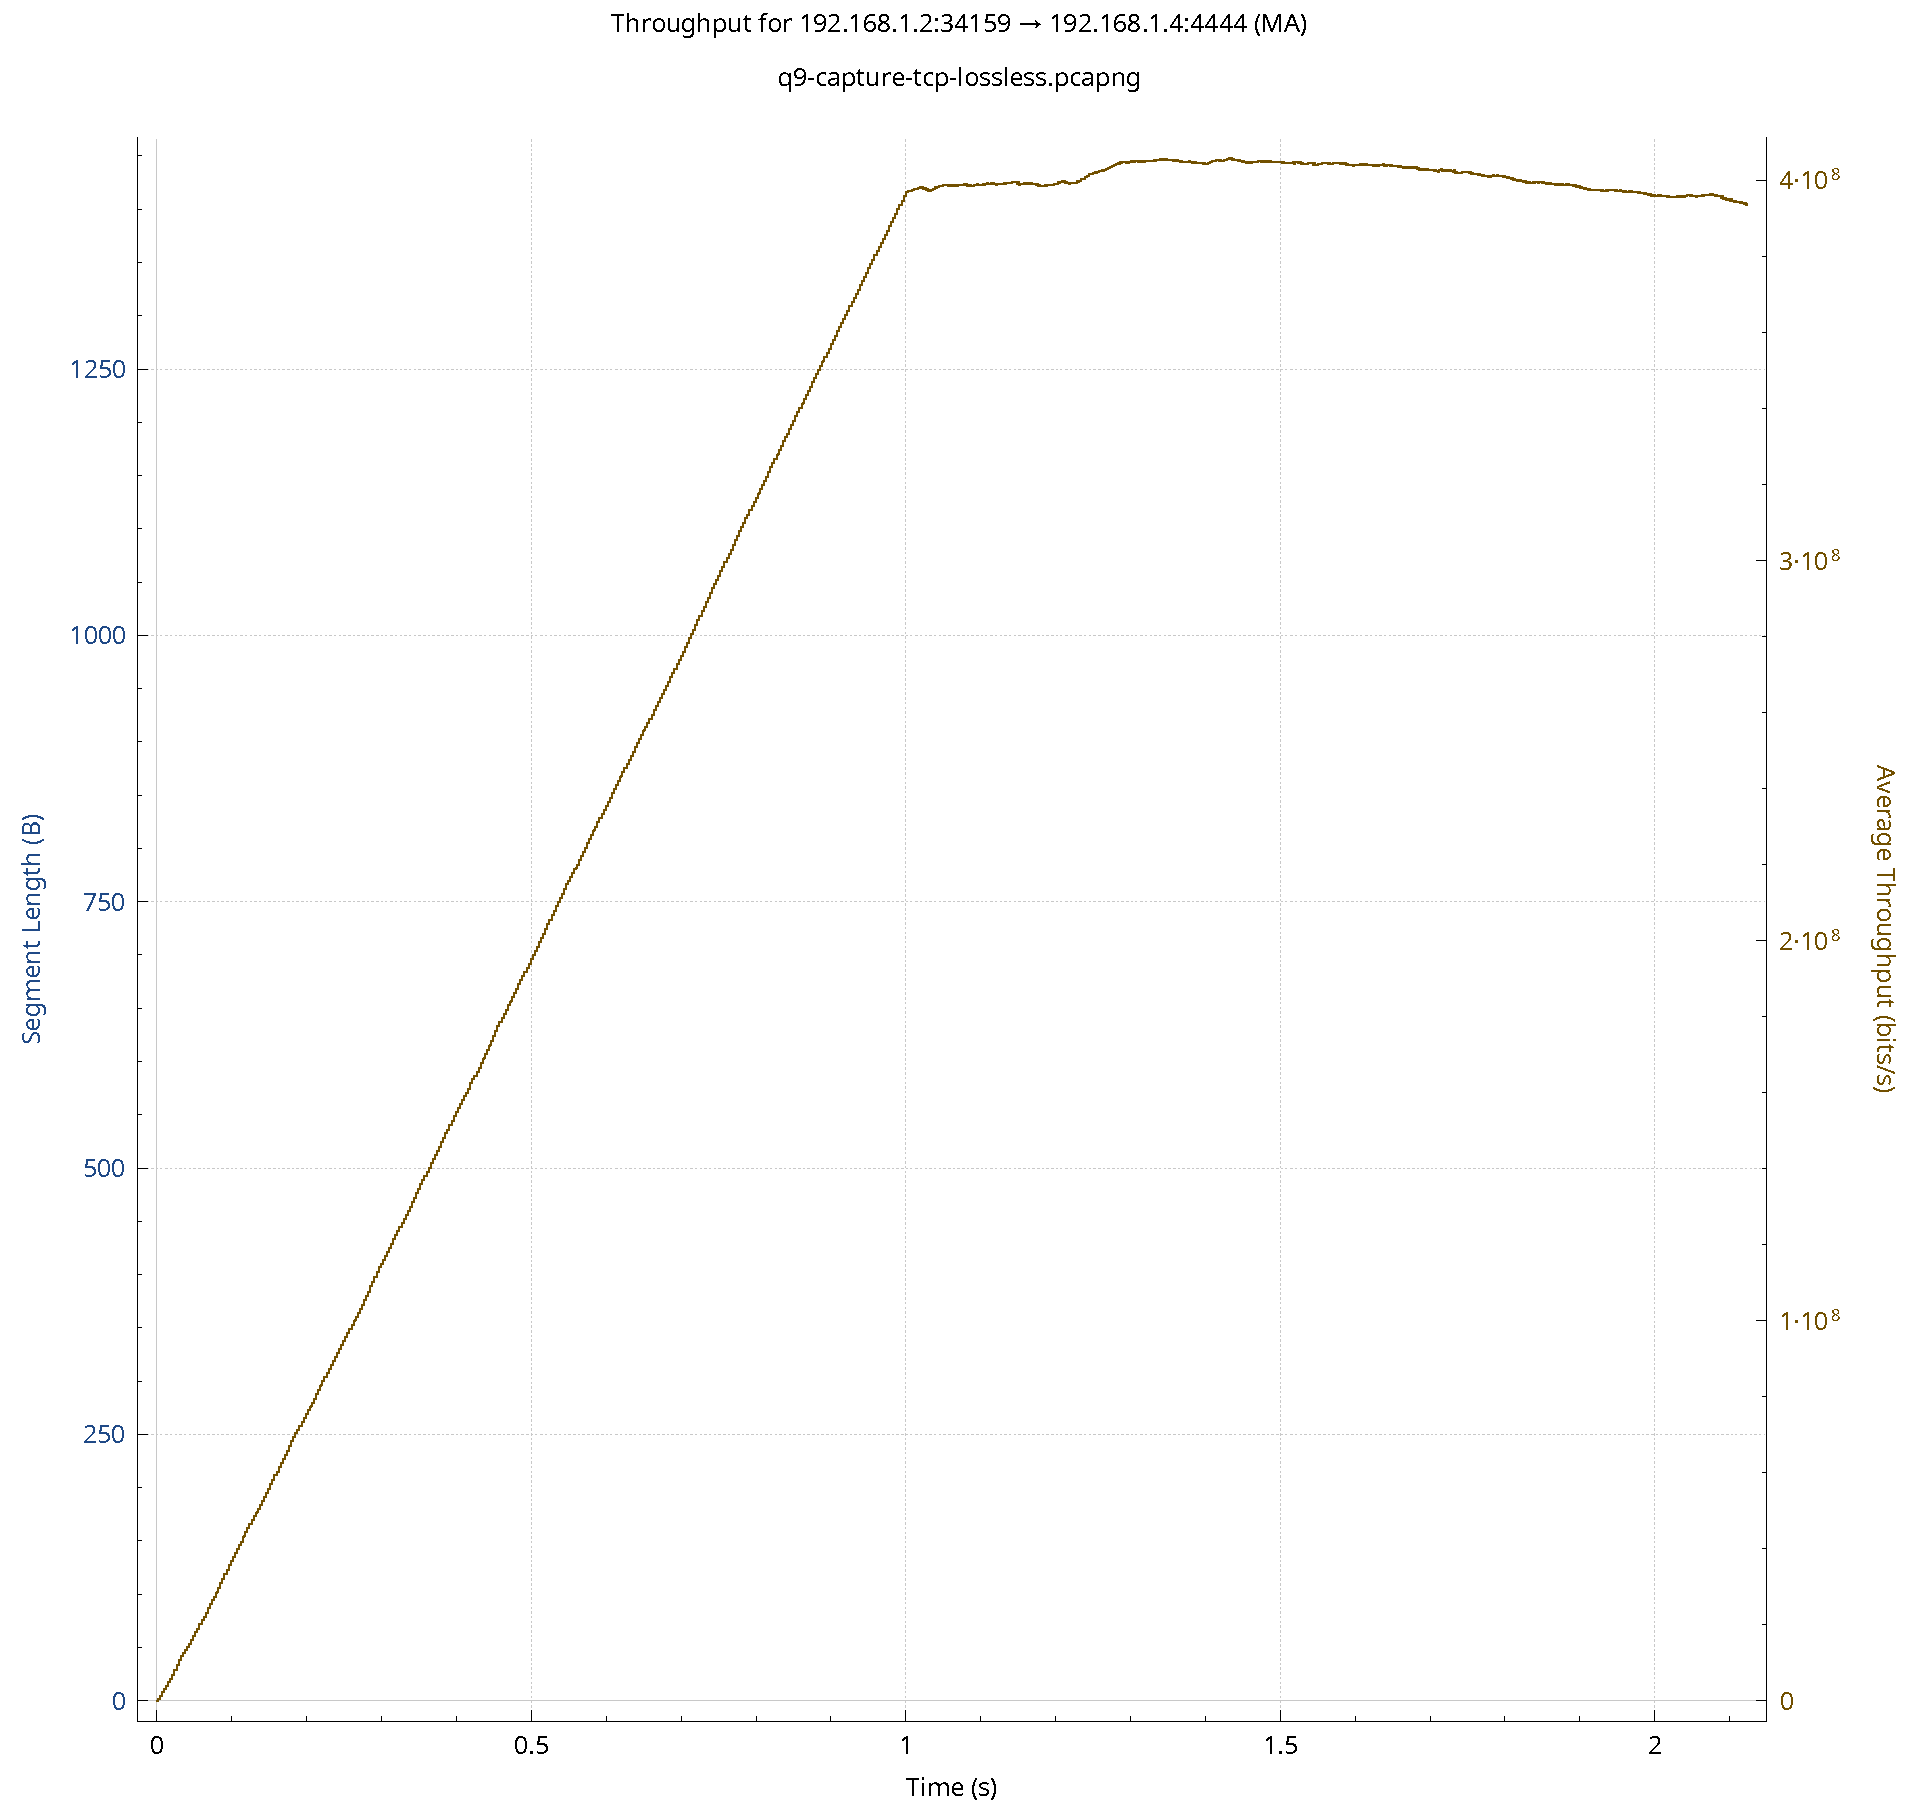
\includegraphics[width=16cm]{data/q9-1msav-throughput.pdf}
\caption{A plot of the 1-second MA of throughput against time
(lossless).}
\label{fig:tcp-lossless}
\end{figure}

\begin{figure}[H]
\centering
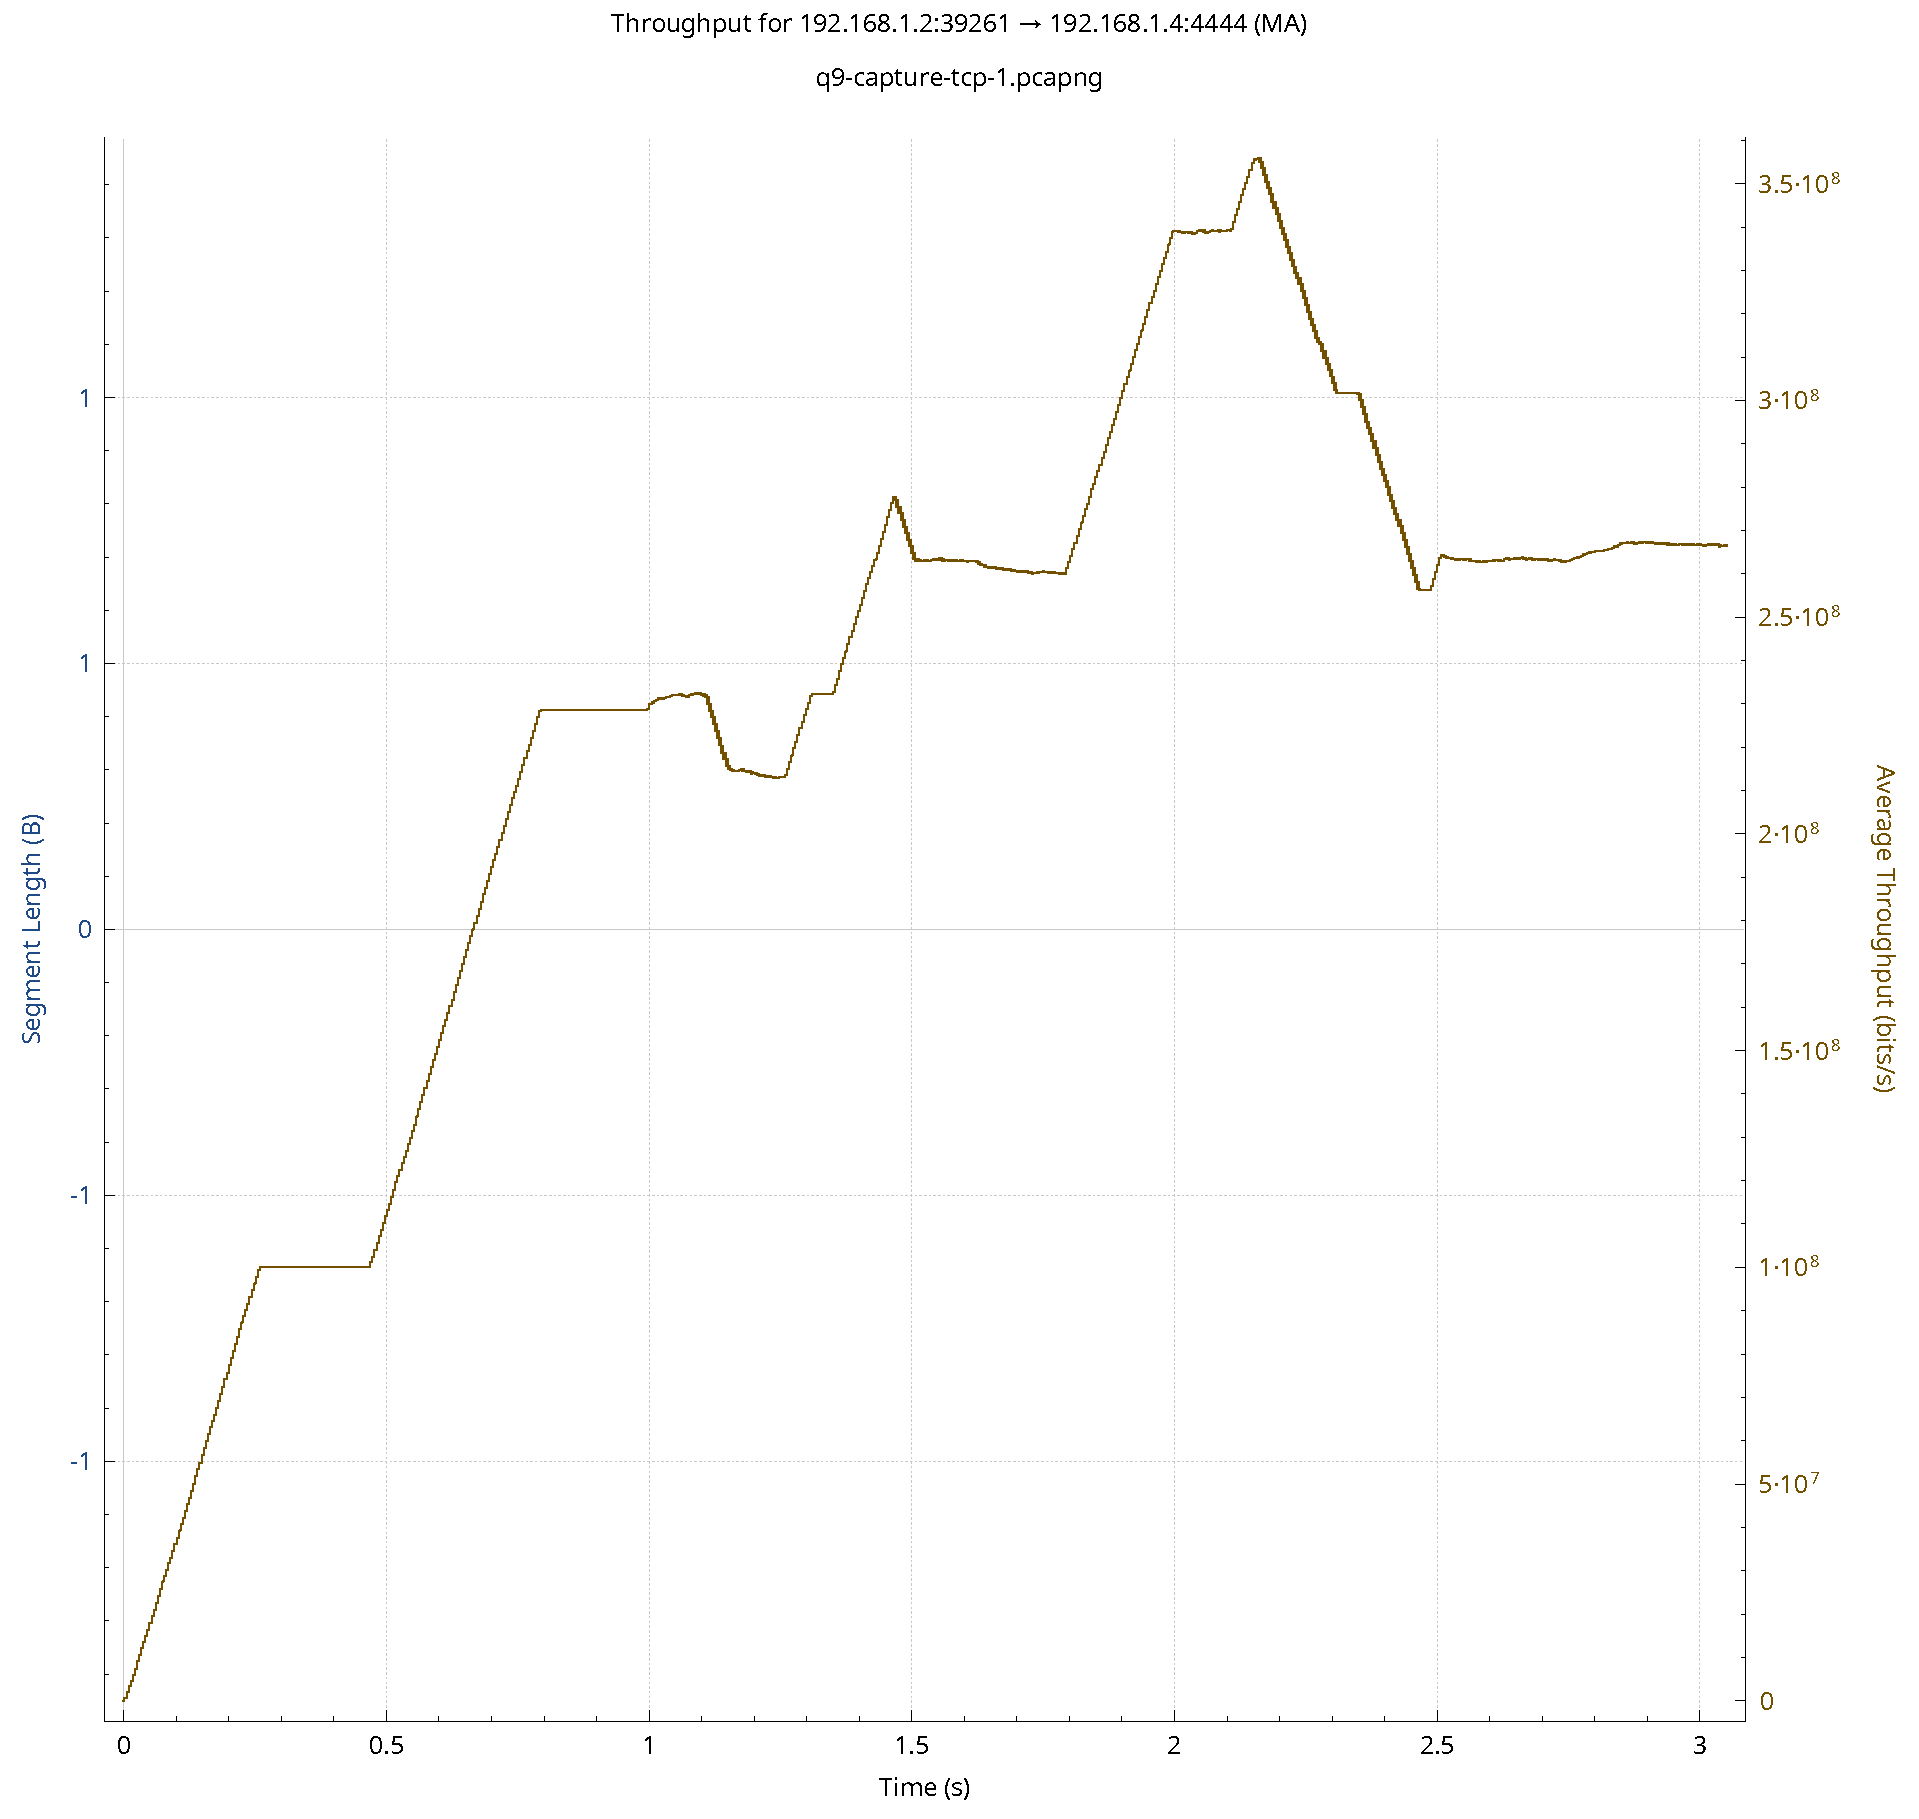
\includegraphics[width=16cm]{data/q9-1msav-throughput-1loss.pdf}
\caption{A plot of the 1-second MA of throughput against time
(1\% loss).}
\label{fig:tcp-1loss}
\end{figure}

\begin{figure}[H]

\centering
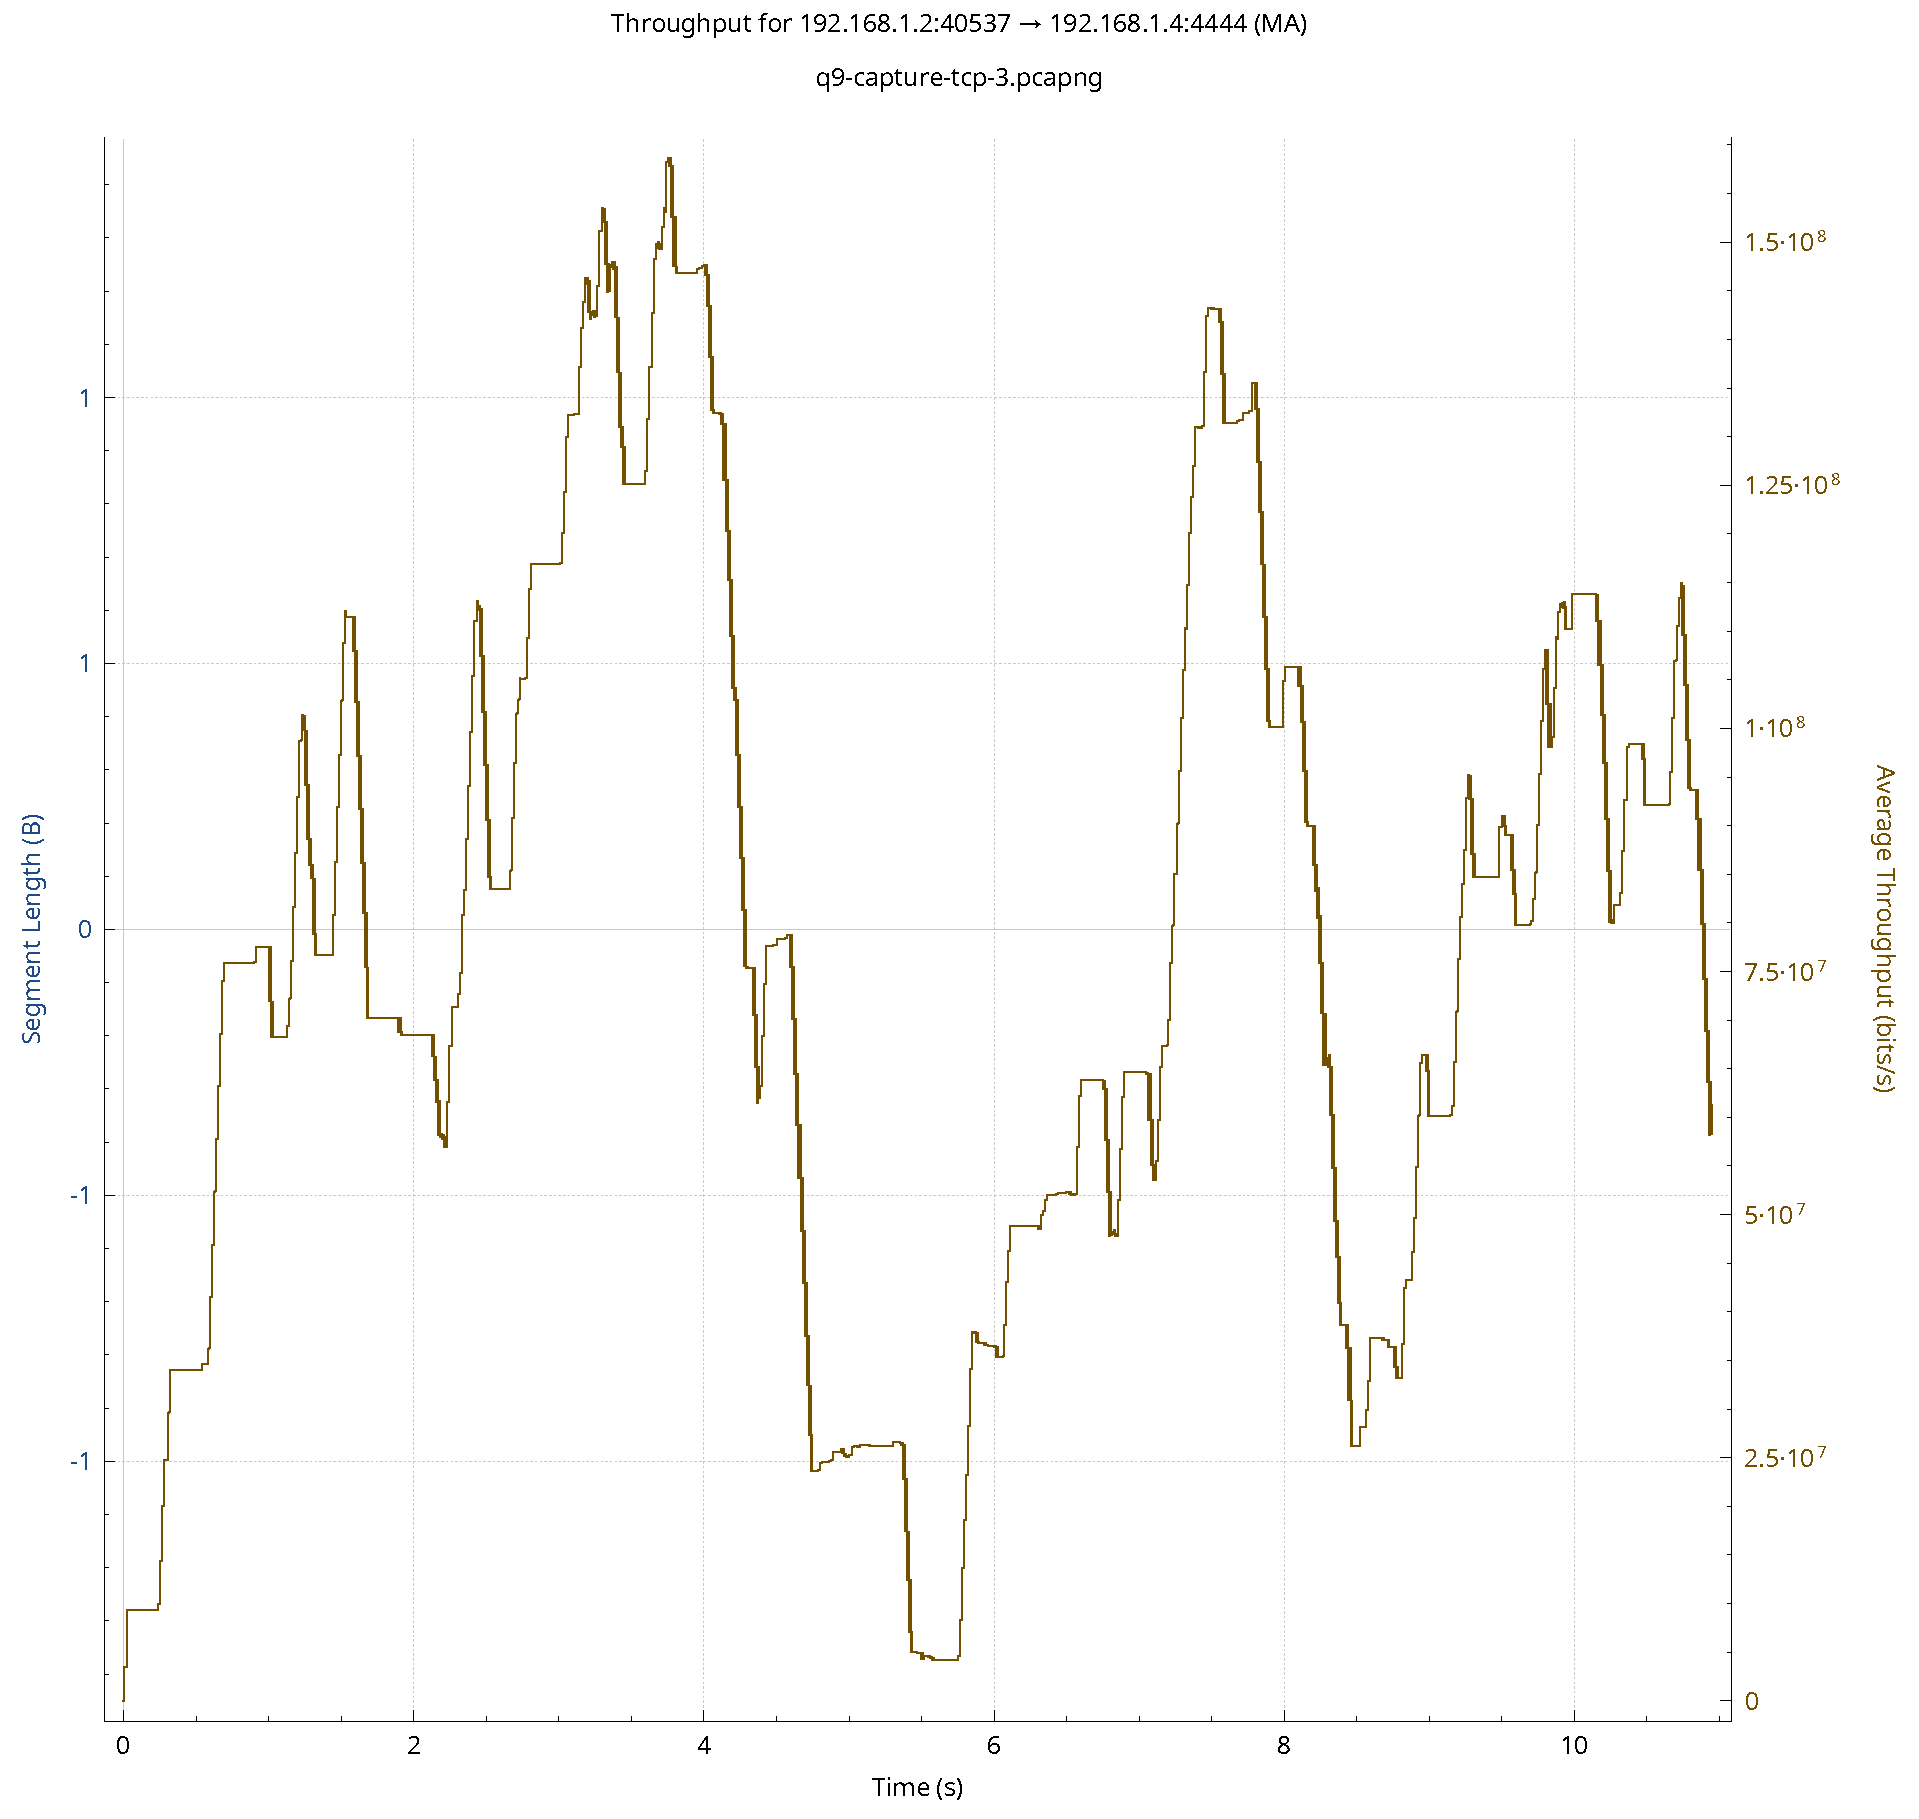
\includegraphics[width=16cm]{data/q9-1msav-throughput-3loss.pdf}
\caption{A plot of the 1-second MA of throughput against time
(3\% loss).}
\label{fig:tcp-3loss}
\end{figure}

\begin{figure}[H]
\centering
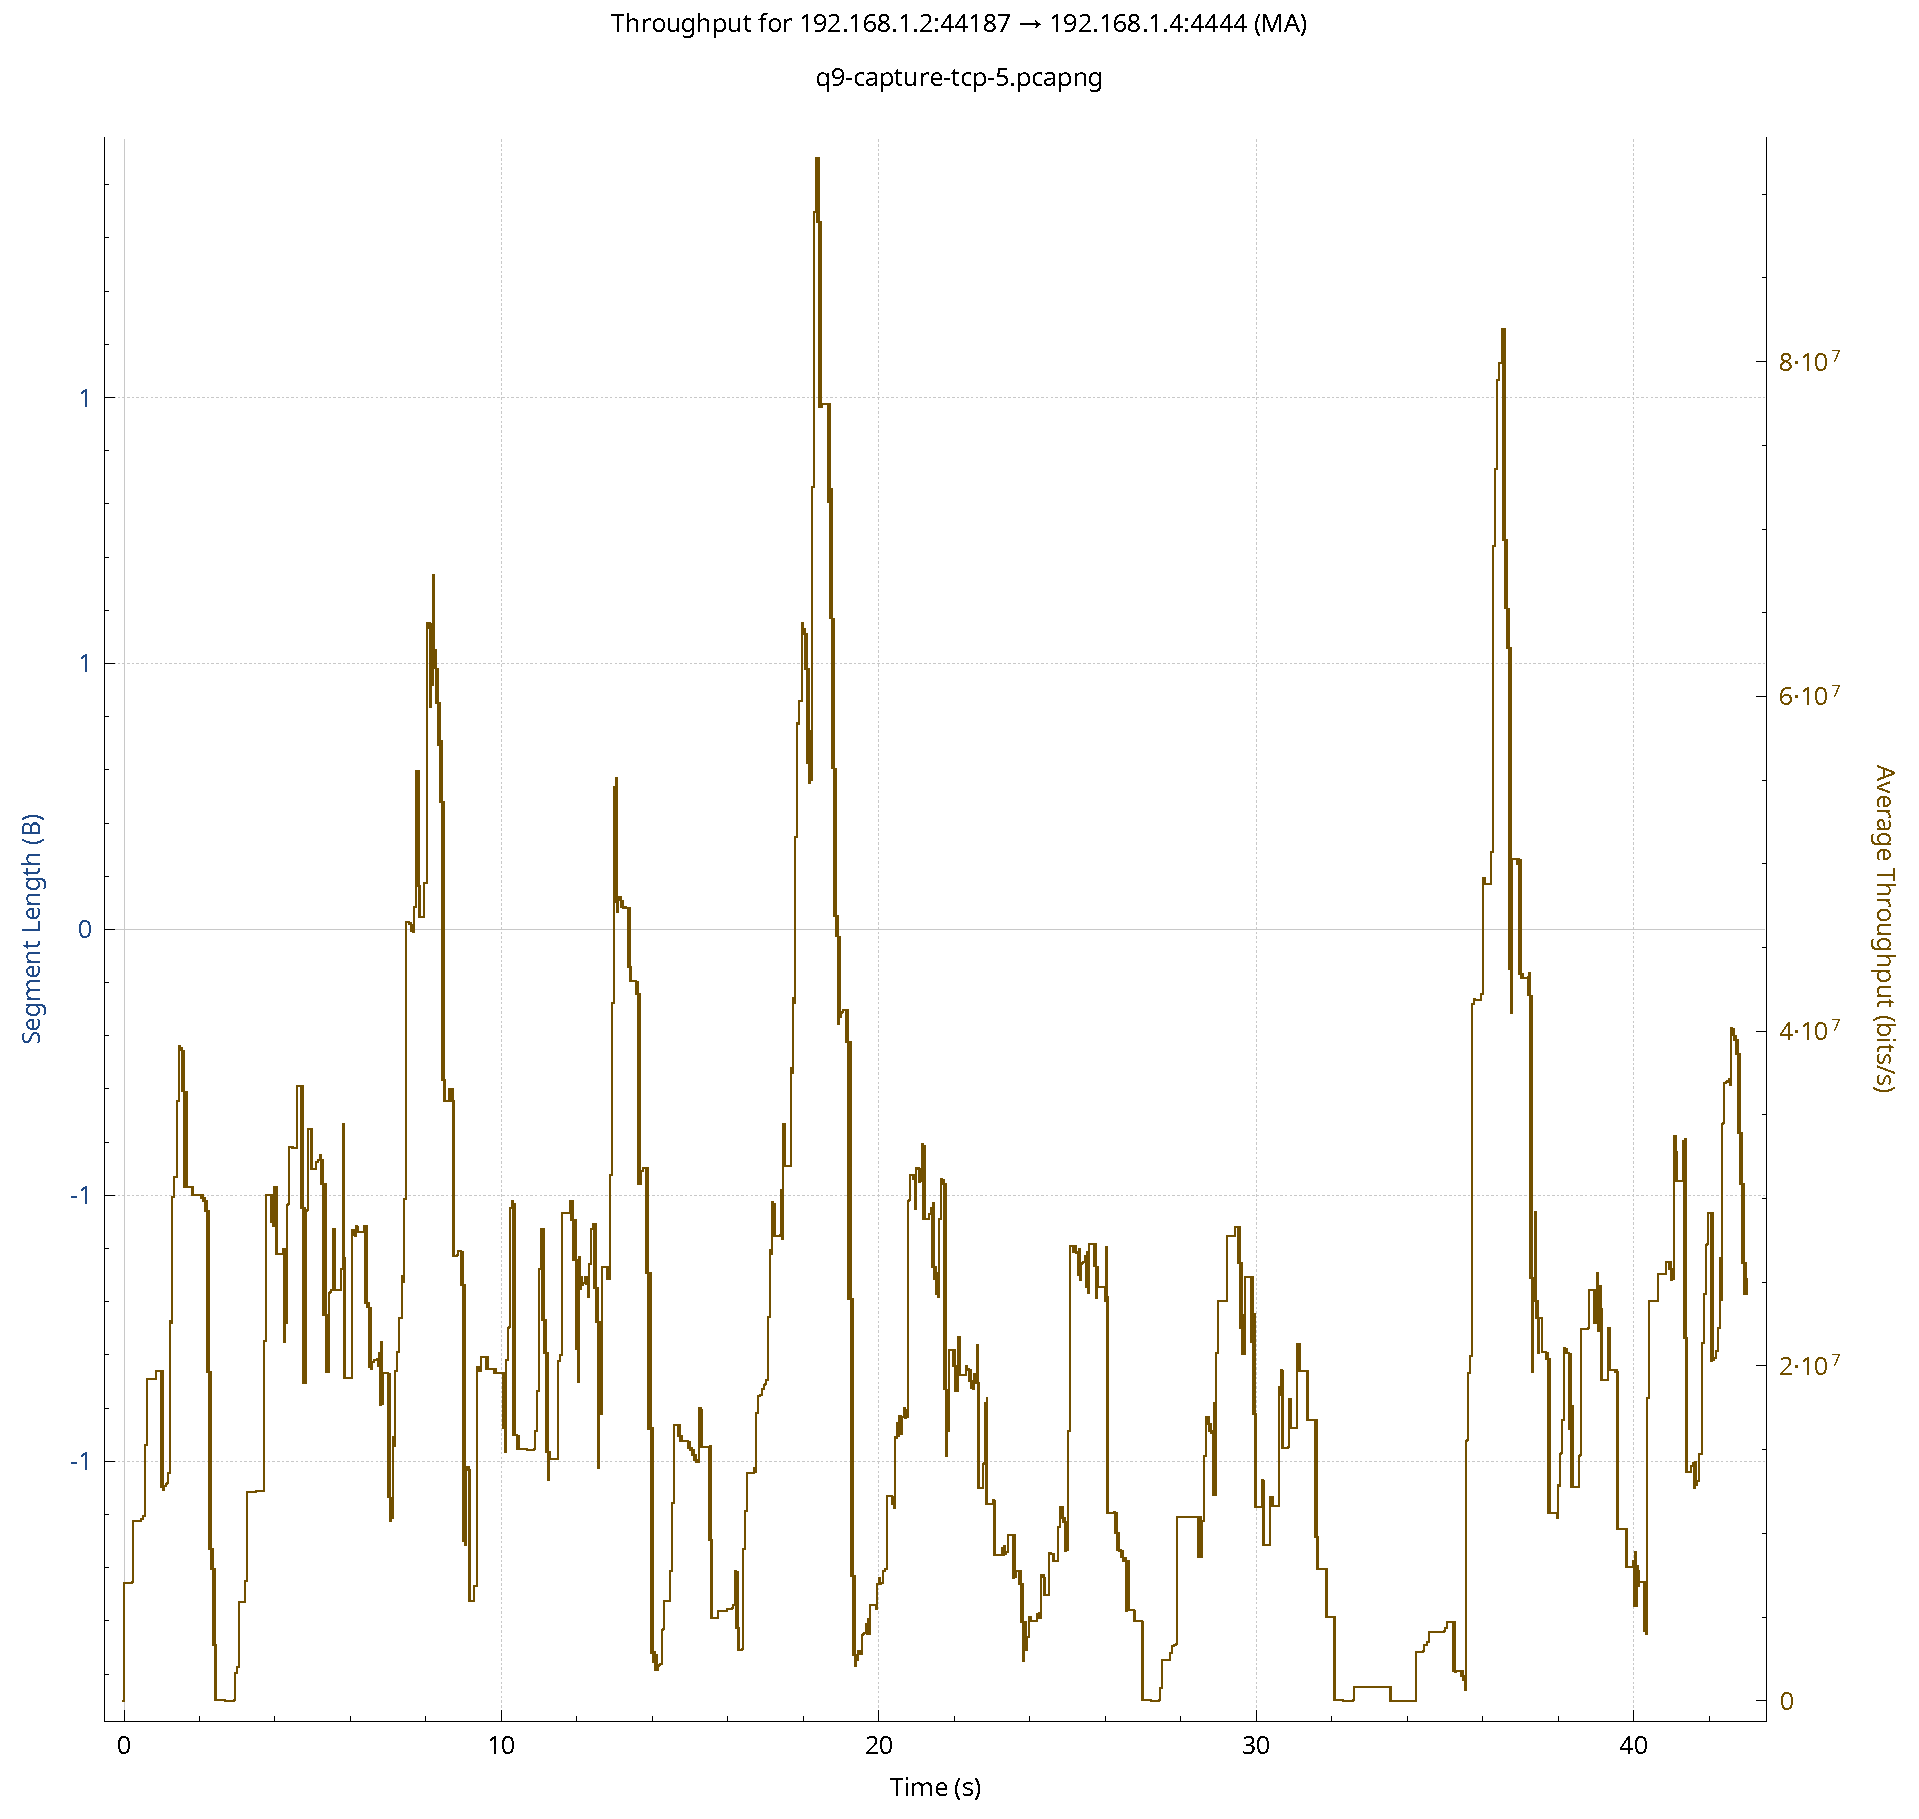
\includegraphics[width=16cm]{data/q9-1msav-throughput-5loss.pdf}
\caption{A plot of the 1-second MA of throughput against time
(5\% loss).}
\label{fig:tcp-5loss}
\end{figure}

Figures \ref{fig:tcp-lossless}, \ref{fig:tcp-1loss},
\ref{fig:tcp-3loss} and \ref{fig:tcp-5loss} are the plots
generated from Wireshark of a 1-second moving average (MA)
of throughput against time. They were generated at
different loss levels as indicated.

\begin{gruvboxlisting}[language=Python,caption={A Python script for computing a
number of statistics about any Wireshark capture.},label={lst:python-scritp}]
import argparse
import csv

def process_csv(file_path): try: with open(file_path, 'r')
as csv_file: reader = csv.reader(csv_file, delimiter=',',
quotechar='"') data = [(float(row[1]), int(row[5])) for row
in [row for row in reader][1:]]

packet_count = len(data) total_size = sum((length for _,
length in data)) start_time = min((time for time, _ in
data)) end_time = max((time for time, _ in data)) diff_time
= end_time - start_time average_throughput =
total_size/diff_time file_size = 100*1024*1024
average_effective_throughput = file_size / diff_time

print( f"""General Info -> Packet Count: {packet_count}
Total Size (in Bytes): {total_size} Start Time (in
Seconds): {start_time} End Time (in Seconds): {end_time}
Difference (in Seconds): {diff_time} Average Throughput (in
Bytes/Second): {total_size}/{diff_time} =
{average_throughput}

Conversions (Throughput) -> Average Throughput (in
MegaBits/Second): {(average_throughput * 8) / (1000 ** 2)}
Average Throughput (in MegaBytes/Second):
{average_throughput / (1000 ** 2)}

Effective Throughput (For 100MibiByte File) -> Average
Effective Throughput (in Bytes/Second):
{file_size}/{diff_time} = {average_effective_throughput}

Conversions (Effective Throughput)-> Average Effective
Throughput (in MegaBits/Second):
{(average_effective_throughput * 8) / (1000 ** 2)} Average
Effective Throughput (in MegaBytes/Second):
{average_effective_throughput / (1000 ** 2)}""")

except FileNotFoundError: print(f"Error: File '{file_path}'
not found.") except Exception as e: print(f"An error
occurred: {e}")

def main(): parser =
argparse.ArgumentParser(description="Process a CSV file.")
parser.add_argument('file', metavar='FILE', help='Path to
the CSV file')

args = parser.parse_args() process_csv(args.file)

if __name__ == "__main__": main()
\end{gruvboxlisting}

Listing \ref{lst:python-scritp}, is Python script used for
computing a number of metrics about any Wireshark capture
which has been converted into a CSV.

Specifically, the captures associated with the above four
figures were converted into CSV files. Then those CSV files
were processed using the above script.

\begin{note}
The CSV files were generated from Wireshark with the following
filter \texttt{tcp.port == 4444 \&\& ip.src == 192.168.1.2} (see
Figure \ref{fig:capture-filter}) to ensure that only
uni-directional throughput is considered.

\begin{figure}[H]
\centering
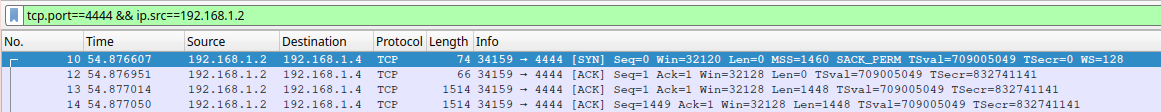
\includegraphics[width=12cm]{data/capture-filter.png}
\caption{A picture of the capture filter active for extracting
the appropriate packets.}
\end{figure}

This is because as mentioned on the Lab Forum, twisted pair
cables are full duplex. This means that traffic can flow in both
directions simultaneously without impacting the throughput of
each direction.
\end{note}

\begin{figure}[H]
\centering
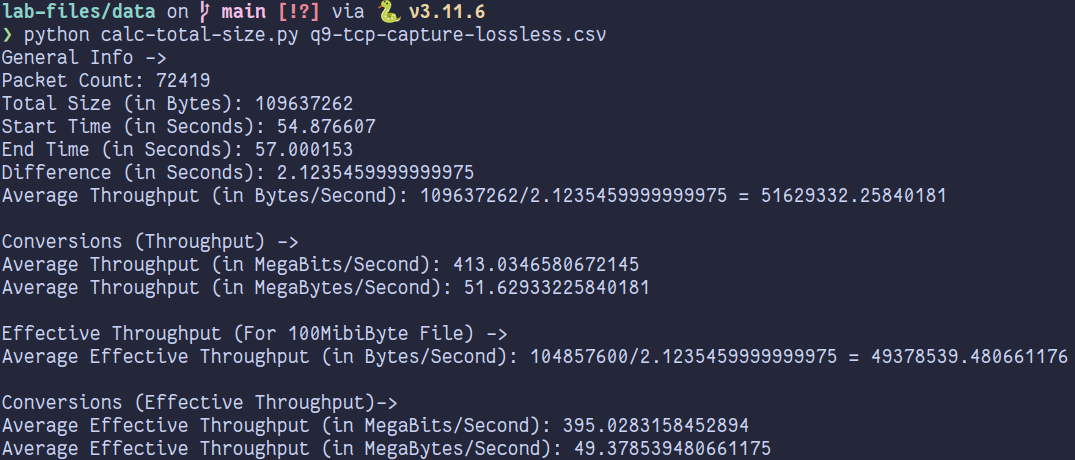
\includegraphics[width=16cm]{data/q9-stats-tcp-lossless.png}
\caption{The statistics generated by the Python script for lossless transfer.}
\end{figure}

\begin{figure}[H]
\centering
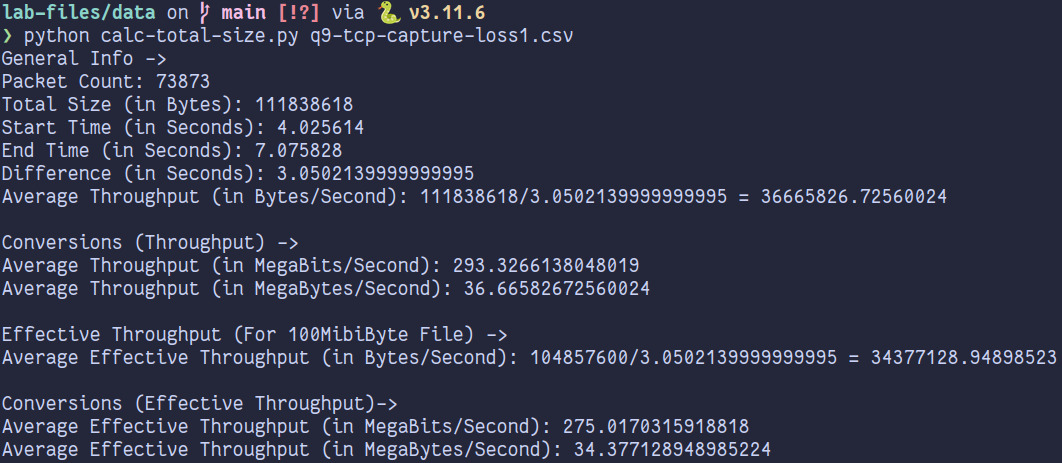
\includegraphics[width=16cm]{data/q9-stats-tcp-loss1.png}
\caption{The statistics generated by the Python script for 1\% loss transfer.}
\end{figure}

\begin{figure}[H]
\centering
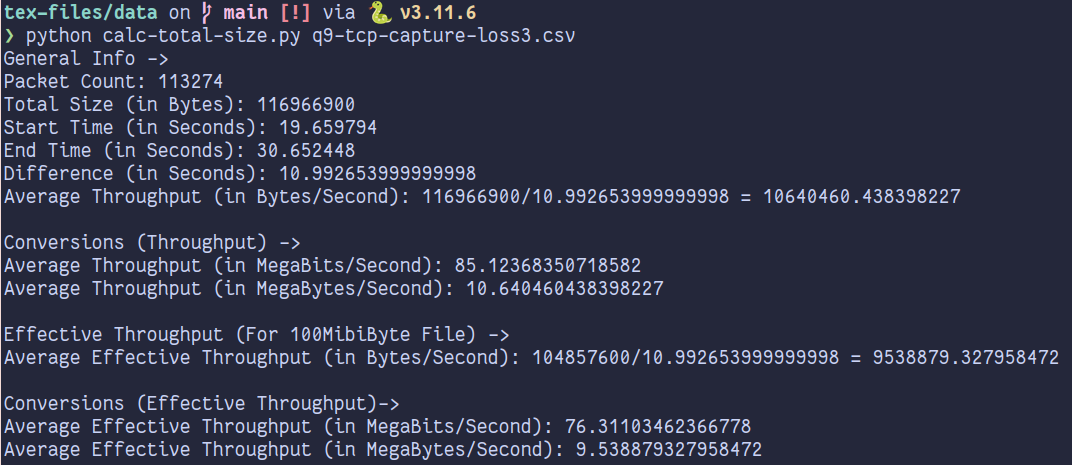
\includegraphics[width=16cm]{data/q9-stats-tcp-loss3.png}
\caption{The statistics generated by the Python script for 3\% loss transfer.}
\end{figure}

\begin{figure}[H]
\centering
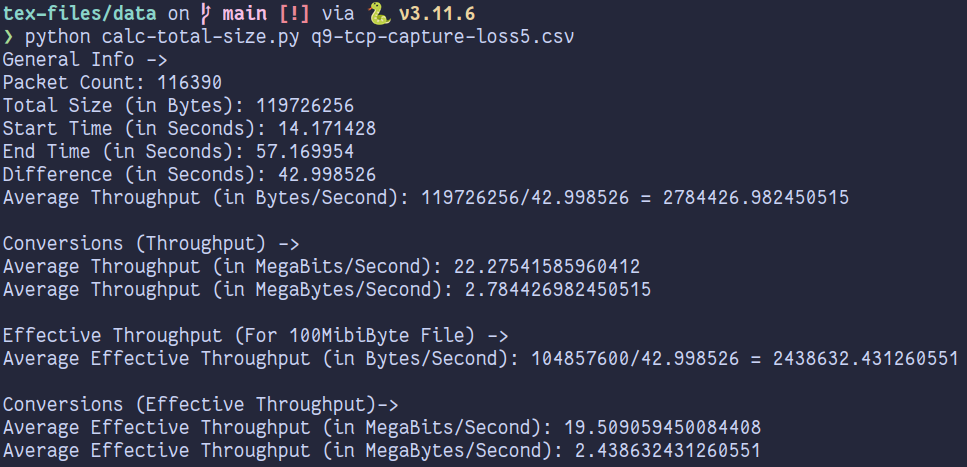
\includegraphics[width=16cm]{data/q9-stats-tcp-loss5.png}
\caption{The statistics generated by the Python script for 5\% loss transfer.}
\end{figure}

\begin{note}
The Python script \texttt{calc-total-size.py} and CSV files used are present in the \texttt{data} directory.
\end{note}

From the above figures the following results can be read.

\begin{center}
\begin{longtable}{c|cc}
\caption{The throughput results generated by the Python script (to two decimal places).}
\label{longtable:results-q9}                                                                            \\
\multicolumn{1}{c|}{}                 &
\multicolumn{1}{c}{Throughput (MB/s)} &
\multicolumn{1}{c}{Effective Throughput (MB/s)}\\
\hline
\endfirsthead

\multicolumn{3}{c}{\tablename\ \thetable{} -- continued from previous page}                                     \\
\hline
\endhead

\hline
\multicolumn{3}{|c|}{{continued on next page}}                                                                  \\
\hline
\endfoot

\endlastfoot

Lossless & 51.63 & 49.38\\
1\% Loss & 36.67 & 34.38\\
3\% Loss & 10.45 & 9.58 \\
5\% Loss & 2.72  & 2.44
\end{longtable}
\end{center}

\begin{note}
A distinction was made between \textbf{throughput} and \textbf{effective
throughput}.

Throughput gives the true throughput of the wire \ie{} how many
raw bytes can be transferred per second over the wire. The
equation is given as follows: $$ \text{Throughput} =
\frac{\text{Total Data (incl. Protocol Overhead)}}{\text{End
Time} - \text{Start Time}} $$ On the other hand, effective
throughput gives the usable or useful throughput of the wire
\ie{} how many bytes of interest to the user (\eg{} a file) can
be transferred per second over the wire \textit{not} factoring
all the bytes used by the underlying transport protocol. $$
\text{Effective Throughput} = \frac{\text{Total Data (excl.
Protocol Overhead)}}{\text{End Time} - \text{Start Time}} $$
\end{note}
\end{ans}

\Que{10}{
Consider the packet sequence pertaining to the lossless case.
\begin{enumerate}
\item List the flags (within square brackets) pertaining to the
      first three packets.
\item What part of connection establishment do the first three
      packets pertain to?
\item List the sequence (Seq=) and acknowledgement (Ack=) numbers
      pertaining to the first three packets.
\item Identify the maximum segment size which the two parties in
      the connection state.
\item Identify the range of packets involved in the data transfer
      phase.
\item Identify the packet(s) involved in the connection teardown
      phase.
\end{enumerate}

\textbf{Show screenshots that allow a reader to validate your answers.}}

\begin{ans}
\begin{figure}[H]
\centering
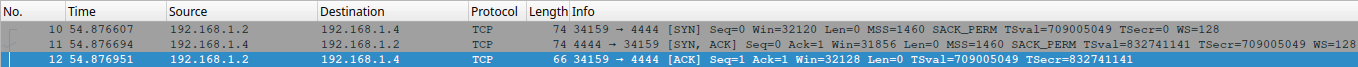
\includegraphics[width=18cm]{data/ans-q10.1.png}
\caption{Screenshot of the first three TCP packets from the lossless capture.}
\label{fig:ans-q10.1}
\end{figure}

\begin{enumerate}
\item \texttt{SYN} for the first packet, \texttt{SYN} and \texttt{ACK} for the
      second packet and finally, \texttt{ACK} for the third packet.
\item These three packets form part of the Three-Way Handshake
      which establishes a reliable connection between the sender
      and receiver.
\item \texttt{Seq} = 0 for the first packet, \texttt{Seq} = 0 and \texttt{Ack} =
      1 for the second packet and finally, \texttt{Seq} = 1 and \texttt{Ack} = 1 for
      the third packet.
\item The maximum segment size (\texttt{MSS}) is 1460 bytes, see
      the second packet.
\end{enumerate}

\begin{figure}[H]
\centering
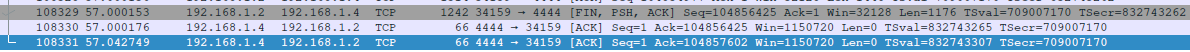
\includegraphics[width=18cm]{data/ans-q10.4.png}
\caption{Screenshot of the last three TCP packets from the lossless capture.}
\label{fig:ans-q10.4}
\end{figure}

\begin{enumerate}
\setcounter{enumi}{4}
\item From Figures \ref{fig:ans-q10.1} \& \ref{fig:ans-q10.4} the
      range of the packets is 10 to 108331.
\item The packets that form part of the teardown are those in
      Figure \ref{fig:ans-q10.4}.
\end{enumerate}
\end{ans}

\Que{11}{
Consider the packet sequence pertaining to the 5\% packet loss
case. List \texttt{received\_file} on alpine-4 and compare its
size with that of \texttt{large\_file}.

\textbf{Show screenshots that allow a reader to validate your
answers.}}
\begin{ans}
\begin{figure}[H]
\centering
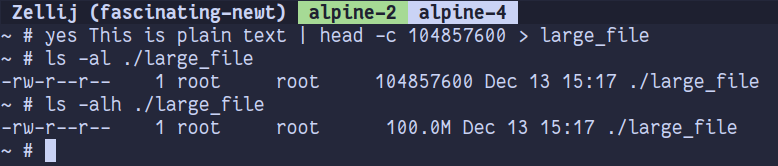
\includegraphics[width=16cm]{data/large-file-alpine-2.png}
\caption{Large file generation on alpine-2.}
\label{fig:file-gen}
\end{figure}

\begin{figure}[H]
\centering
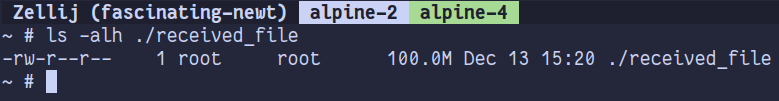
\includegraphics[width=16cm]{data/alpine-4-received-file.png}
\caption{Listing received large file on alpine-4.}
\label{fig:file-receive}
\end{figure}

As can be seen from Figures \ref{fig:file-gen} \&
\ref{fig:file-receive} the file size remained the same. This is
the case because TCP is a reliable data transport protocol \ie{}
it provides a zero-tolerance policy for data loss.
\end{ans}

\newpage

\Que{12}{
Consider the packet sequence pertaining to the lossless case.
\begin{enumerate}
\item List \texttt{received\_file} on alpine-4 and compare its
      size with that of \\ \texttt{large\_file}.
\item Go to File->Export Packet Dissections, export the captured
      packets as CSV and inspect the CSV file in Excel. How does
      the number of octets sent (as you determine from the CSV
      file) compare with the size of\\ \texttt{received\_file}?
\item Inspect the first few packets in the UDP window and
      identify the length of the UDP datagram (``Len''). How does
      this compare with the Ethernet frame's MTU of 1500? Explain
      any difference you observe.
\end{enumerate}

\textbf{Show screenshots that allow a reader to validate your answers.}}

\begin{ans}
\begin{figure}[H]
\centering
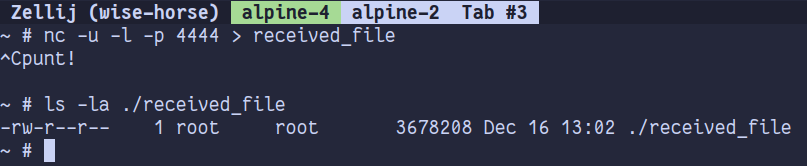
\includegraphics[width=16cm]{data/q12-received-file.png}
\caption{Listing received large file on alpine-4 for Question 12.1.}
\end{figure}

The \texttt{received\_file} in alpine-4 has a size of
3678208 bytes. This is roughly $100 \times
\frac{3678208}{104857600} \approx 3.5\%$ of the original
size of \texttt{large\_file}.

\begin{note}
This seems to be a consequence of using GNS3 with two Docker
containers.  It might be related to the fact that Netcat does
not allow enough time for the packets to be sent. Instead it
tries to send all packets at once which causes Linux in the
Docker containers or the Docker containers themselves to drop a
significant amount of the packets generated by Netcat.

\begin{figure}[H]
\centering
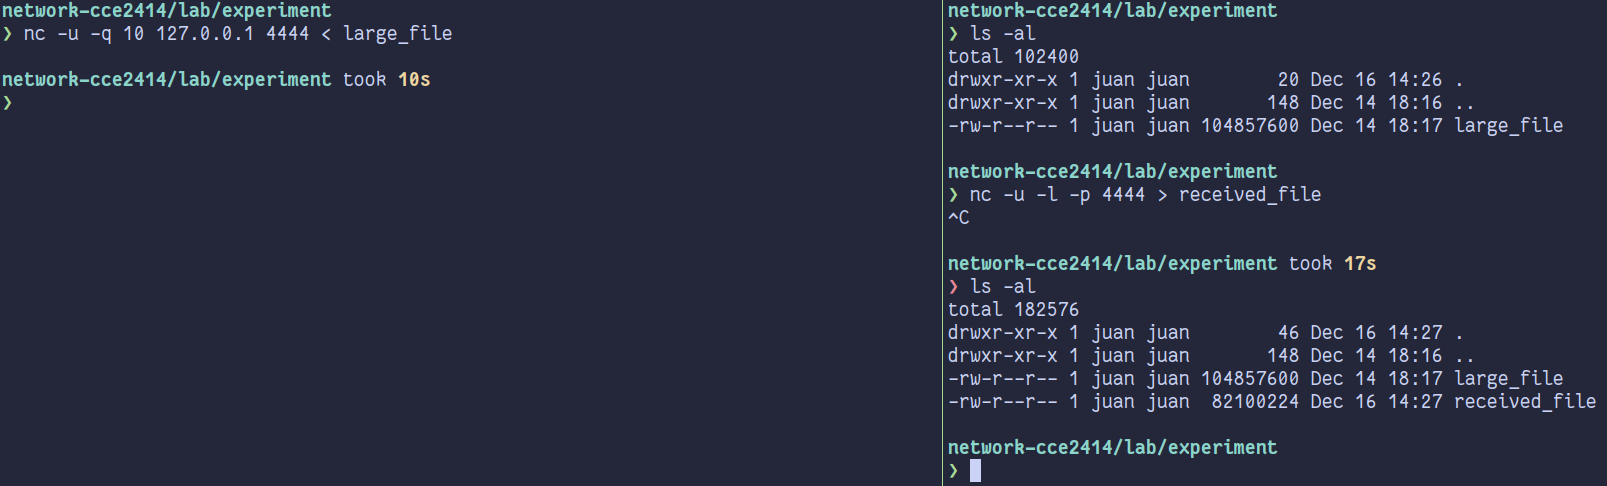
\includegraphics[width=13cm]{data/local-experiment.png}
\caption{Using Netcat in UDP mode for local file transfer using the Loopback
device.}
\label{fig:experiment}
\end{figure}

As can be seen from Figure \ref{fig:experiment} the size of
\texttt{received\_file} is 82100224 bytes. This is $100
\times \frac{82100224}{104857600} \approx 78.3\%$ of the
original file size; a better and more expected
outcome. Additionally, there is also the possibility that
BusyBox Netcat has different behavior from OpenBSD Netcat.
Also extra care was taken to ensure that no mistake was
made and that artificial packet loss was reset to 0\%.
\vspace{1em}
\begin{center}
\textit{Please zoom in onto Figure \ref{fig:experiment} for improved
clarity.}
\end{center}
\end{note}

For the second part of the question again a Python script
similar to Listing \ref{lst:python-scritp} is used. The
only difference is that the size of UDP payloads is assumed
to be exactly 8192 bytes.
\begin{gruvboxlisting}[language=Python, caption={A Python script for computing a
number the total size of a number of maximum size (8192 bytes) UDP packets.}]
import argparse
import csv

def process_csv(file_path): try: with open(file_path, 'r')
as csv_file: reader = csv.reader(csv_file, delimiter=',',
quotechar='"') data = [(float(row[1]), int(row[5])) for row
in [row for row in reader][1:]]

packet_count = len(data) total_size = 8192 * packet_count
start_time = min((time for time, _ in data)) end_time =
max((time for time, _ in data)) diff_time = end_time -
start_time

print( f"""General Info -> Packet Count: {packet_count}
Total Size (in Bytes): {total_size} Start Time (in
Seconds): {start_time} End Time (in Seconds): {end_time}
Difference (in Seconds): {diff_time}

Conversions -> Total Size (in MibiBytes): {(total_size) /
(1024 ** 2)}""")

except FileNotFoundError: print(f"Error: File '{file_path}'
not found.") except Exception as e: print(f"An error
occurred: {e}")

def main(): parser =
argparse.ArgumentParser(description="Process a CSV file.")
parser.add_argument('file', metavar='FILE', help='Path to
the CSV file')

args = parser.parse_args() process_csv(args.file)

if __name__ == "__main__": main()
\end{gruvboxlisting}

\begin{note}
The Python script \texttt{udp-total-size.py} and CSV file used
are present in the \texttt{data} directory.
\end{note}

\begin{figure}[H]
\centering
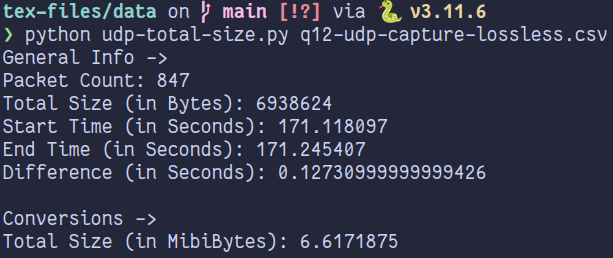
\includegraphics[width=13cm]{data/q12-udp-capture-stats.png}
\caption{Information about the UDP Wireshark capture (lossless).}
\label{fig:q12-udp-capture-info}
\end{figure}

Again, these calculations where made under the assumption
that the \texttt{Len} information provided by the UDP
packets should be used to identify the length of the UDP
payload. From Figure \ref{fig:q12-udp-capture-info} the
total size of useful data captured is roughly 6.6 MibiBytes
which is not the size of the \texttt{received\_file} (3.6
MibiBytes). Hence, the only reasonable conclusion is that
there has been some additional loss exactly upon receipt at
alpine-4.

Finally, the \texttt{Len} UDP is field is set to 8192. This
value is clearly greater than the 1500 bytes, which is the
Maximum Transfer Unit (MTU) of an Ethernet frame. This is
not contradicting the size restriction imposed at layer 2.
UDP has not awareness of what is happening layer 3 and
below. Hence, the whole UDP is actually dismantled into
separate smaller chunks which respect the MTU and then
these IP packets are reorder and recombined to reconstruct
the UDP packet. This is also indicated to us by Wireshark,
see Figure \ref{fig:q12-udp-packet-reassembly}.

\begin{figure}[H]
\centering
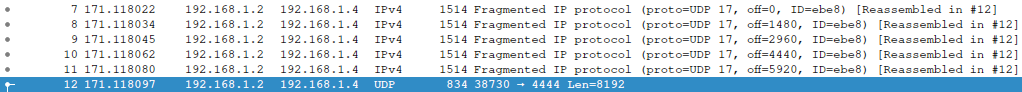
\includegraphics[width=16cm]{data/ip-reconstruction.png}
\caption{A subsection of the UPD Wireshark capture demonstrating packet
reassembly.}
\label{fig:q12-udp-packet-reassembly}
\end{figure}
\end{ans}

\Que{13}{Explain the difference between your observations in 11
and 12.1.}
\begin{ans}
The major take away from the answers to questions 11 and 12 is
that TCP and UDP are very different in their approach. TCP is
considered to be connection-oriented and reliable. This is
because TCP ensures that data is not lost, not corrupted and
totally delivered. This is even the case when the network is not
stable (as simulated in question 11 with a 5\% packet loss
rate).

On the other hand, UDP is known as a stateless and
connection-less data transfer protocol. This is because UDP does
not give any guarantees about the reliability of data transfer.
In fact, it is possible that none of the data sent over UDP,
actually reaches its intended destination. Additionally, UDP
does not even attempt to check whether the recipient of the data
is available to receive.

In fact, Netcat will work when started in UDP mode even
when no recipient is available. However, in TCP mode Netcat
will actually exit if the Three-Way Handshake for
connection establishment fails.

However, there are some applications which benefit from UDP.
This is because UDP is a much leaner protocol due to reduced
protocol overhead. Being leaner implies a greater effective
throughput \ie{} it can transfer data at faster rate. 

UDP is leaner because of the fact that it does not need to
establish a connection and more importantly it does not need to
maintain said connection. This makes UDP more suited for
applications with continuous streams of data generation which
are tolerant of some missing data and require low-latency. The
best examples of this are multi-player first-person shooters
(type of games). This is because accuracy within the data is not
required and the same data is often set multiple times.

Finally, to not leave TCP out, it unsurprisingly has a many more
applications since it is the backbone of just about any form of
reliable transfer: file transfers, emails, HTTP (and by proxy
web pages) and more.
\end{ans}
\end{document}
